\section{Results}
\label{results}

Table~\ref{yields} shows the expected number of background events and the observed data in each SR and \pt bin, for each channel. We split SR I into two bins. In the $\Pe\Pgm$ and $\Pgm\Pgm$ channels, these bins are in the leading muon \pt, and in the $\Pe\Pe$ channel, these bins are in the leading electron \pt. The \pt bins, which are defined in Table~\ref{pt_bins}, are chosen such that the high-\pt bin contains less than one background event, which increases the sensitivity to small lifetimes and large masses. As summarized in Fig.\ref{yields_figure}, the observed number of events are consistent with the predicted amount of background.

\begin{table}[ht] 
\noindent \centering{}
\topcaption{The \pt boundaries between the low- and high-\pt bins of SR I in each channel.}
\label{pt_bins}
\begin{tabular}{llll}
\hline
  & \pt boundary [\si{\GeV}] \\
\hline
2016 $\Pe\Pgm$       & leading $\Pgm$ $\pt=90$ \\
2017+2018 $\Pe\Pgm$  & leading $\Pgm$ $\pt=140$ \\
2016 $\Pe\Pe$        & leading $\Pe$ $\pt=300$ \\
2017+2018 $\Pe\Pe$   & leading $\Pe$ $\pt=400$ \\
2016 $\Pgm\Pgm$      & leading $\Pgm$ $\pt=100$ \\
2017+2018 $\Pgm\Pgm$ & leading $\Pgm$ $\pt=100$ \\
\hline
\end{tabular}
\end{table}
\begin{table}
\renewcommand{\arraystretch}{1.3}
\noindent \centering{}
\topcaption{The number of estimated background and observed events in each channel and SR. For each estimate, the total uncertainty is given. The \pt boundaries that separate the low- and high-\pt bins of SR I are listed in Table~\ref{pt_bins}.}
\label{yields}
\begin{tabular}{llllll}
\hline
 & SR I, & SR I,  &  &  & \\
 & low \pt & high \pt & SR II & SR III & SR IV \\
 & bin & bin &  & & \\
\hline
\textit{2016 $\Pe\Pgm$}\\
- estimated        & $3.8^{+4.8}_{-3.8}$    & $0.41^{+0.53}_{-0.41}$ & $0.09^{+0.12}_{-0.09}$ & $0.15\pm0.15$ & $0.003^{+0.004}_{-0.003}$\\
- observed         & 8 & 1 & 0 & 0 & 0\\

\textit{2017+2018 $\Pe\Pgm$}\\
- estimated        & $38\pm13$          & $0.75^{+0.41}_{-0.34}$ & $0.23^{+0.27}_{-0.23}$ & $0.71^{+0.76}_{-0.71}$ & $0.01^{+0.02}_{-0.01}$\\
- observed         & 28 & 3 & 0 & 1 & 0\\

\textit{2016 $\Pe\Pe$}\\
- estimated        & $18\pm11$  & $0.22^{+0.17}_{-0.16}$ & $0.51^{+1.02}_{-0.51}$ & $0.43^{+0.85}_{-0.43}$ & $0.01^{+0.02}_{-0.01}$\\
- observed         & 40 & 0 & 0 & 1 & 0\\

\textit{2017+2018 $\Pe\Pe$}\\
- estimated        & $62^{+18}_{-17}$       & $0.85^{+0.33}_{-0.35}$ & $2.8\pm1.1$            & $3.6\pm1.4$            & $0.24^{+0.10}_{-0.09}$\\
- observed         & 48 & 0 & 1 & 4 & 0\\

\textit{2016 $\Pgm\Pgm$}\\
- estimated        & $7.4\pm3.0$            & $0.25\pm0.11$          & $0.17\pm0.11$          & $0.19\pm0.12$          & $0.01\pm0.01$\\
- observed         & 15 & 0 & 0 & 1 & 0\\

\textit{2017+2018 $\Pgm\Pgm$}\\
- estimated        & $3.5\pm1.5$            & $0.69\pm0.31$          & $0.08^{+0.12}_{-0.08}$ & $0.14^{+0.19}_{-0.14}$ & $0.01^{+0.02}_{-0.01}$\\
- observed         & 1 & 1 & 1 & 1 & 0\\
\hline
\end{tabular}
\end{table}

\begin{figure}
\centering
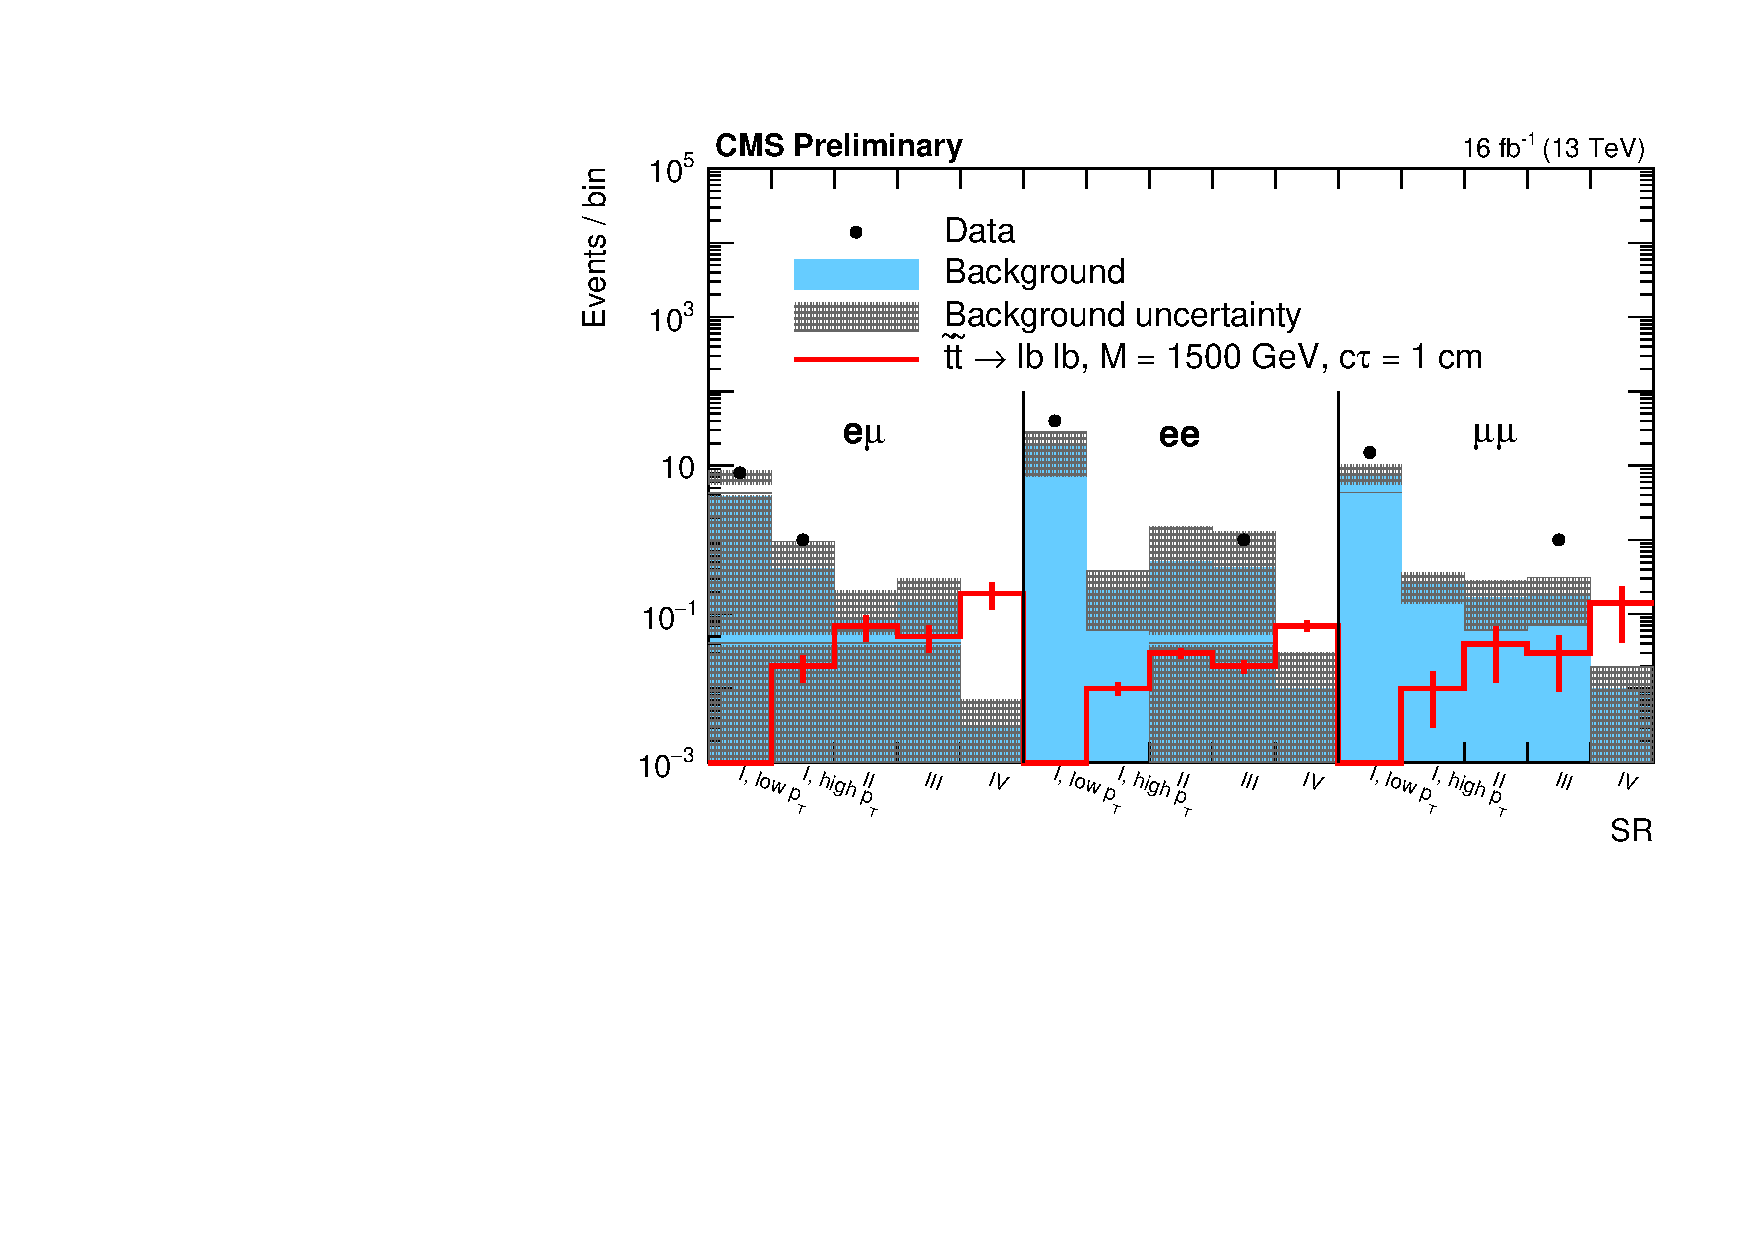
\includegraphics[width=0.8\textwidth]{figures/results/SR2016yields_CMSPreliminary.pdf}
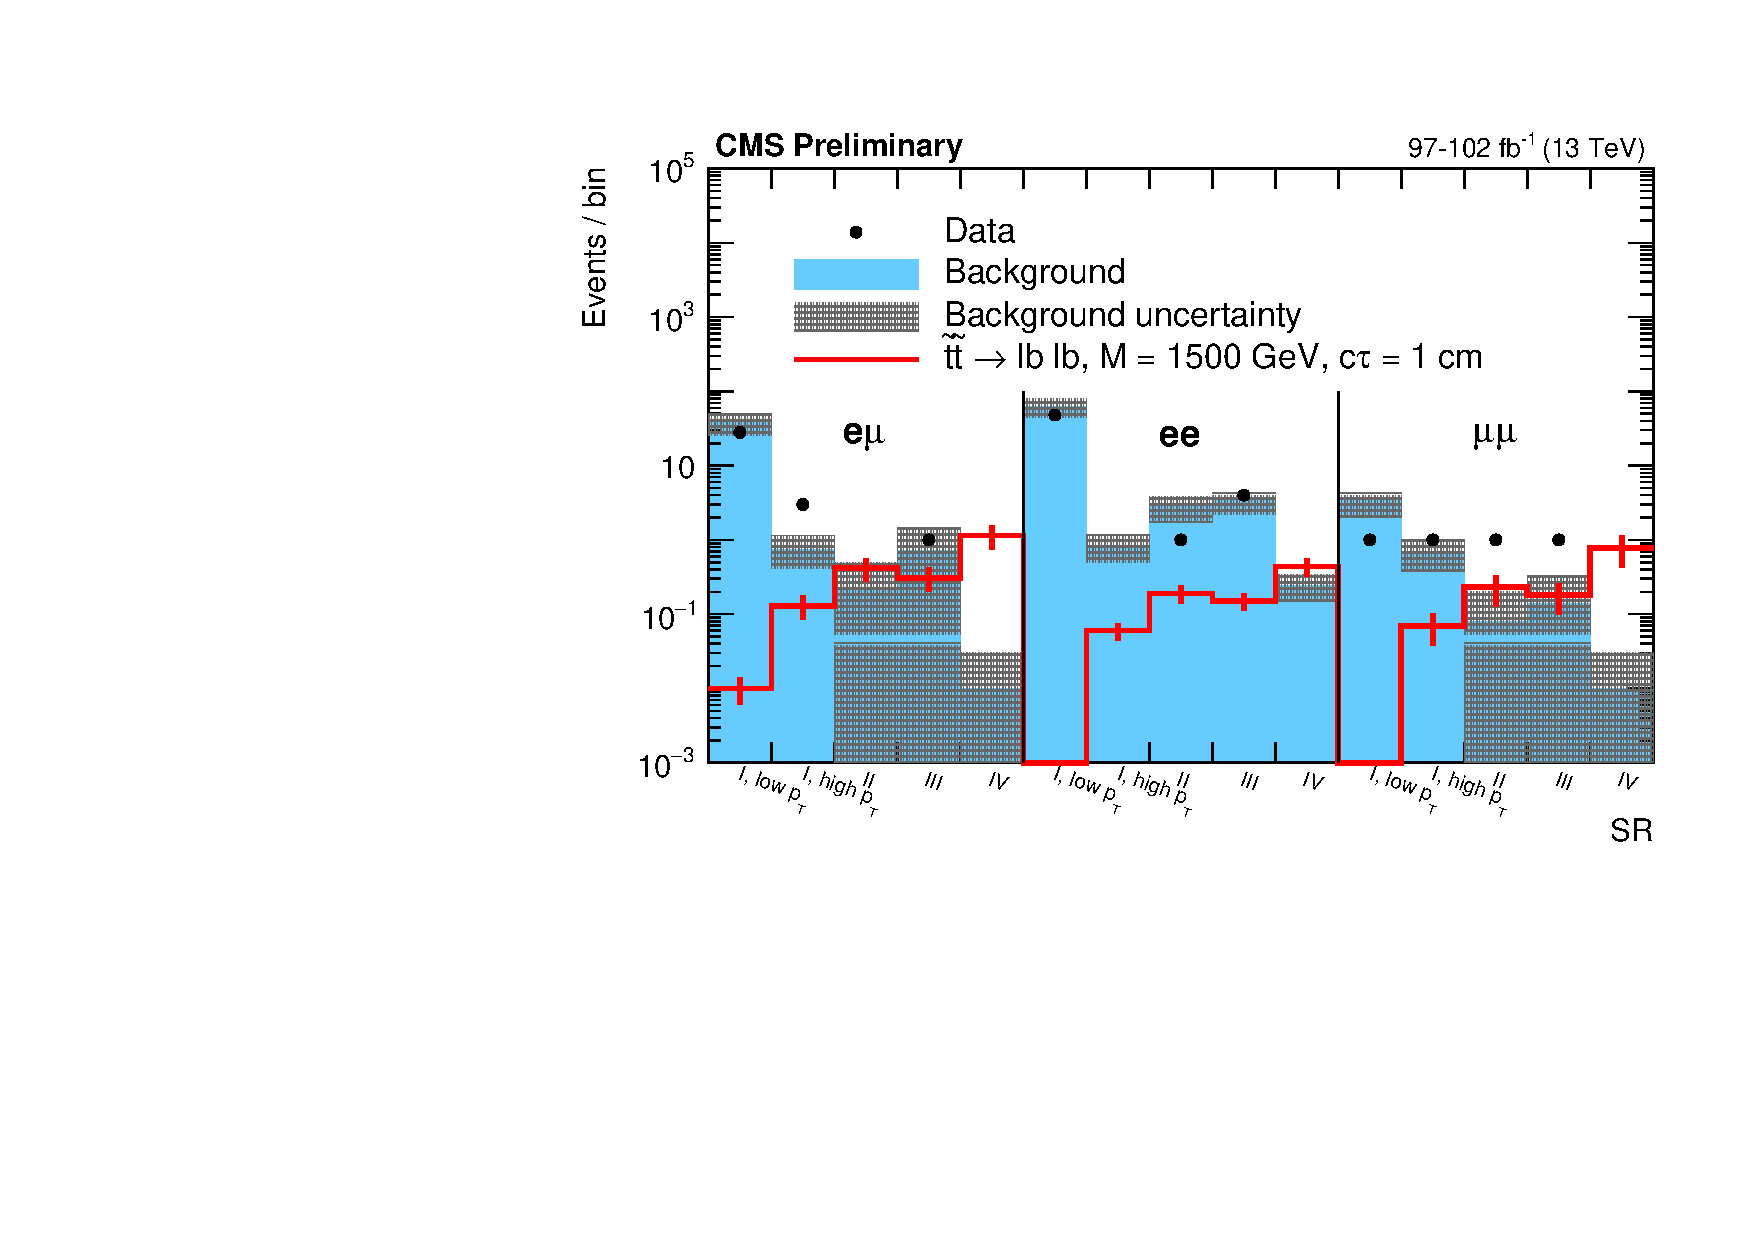
\includegraphics[width=0.8\textwidth]{figures/results/SR201718yields_CMSPreliminary.pdf}
\caption{The number of estimated background and observed events in each channel and SR, with a representative signal overlaid, for 2016 (top) and 2017--2018 (bottom). For each background estimate and signal yield, the total uncertainty is given.}
\label{yields_individual}
\end{figure}

\begin{figure}
\centering
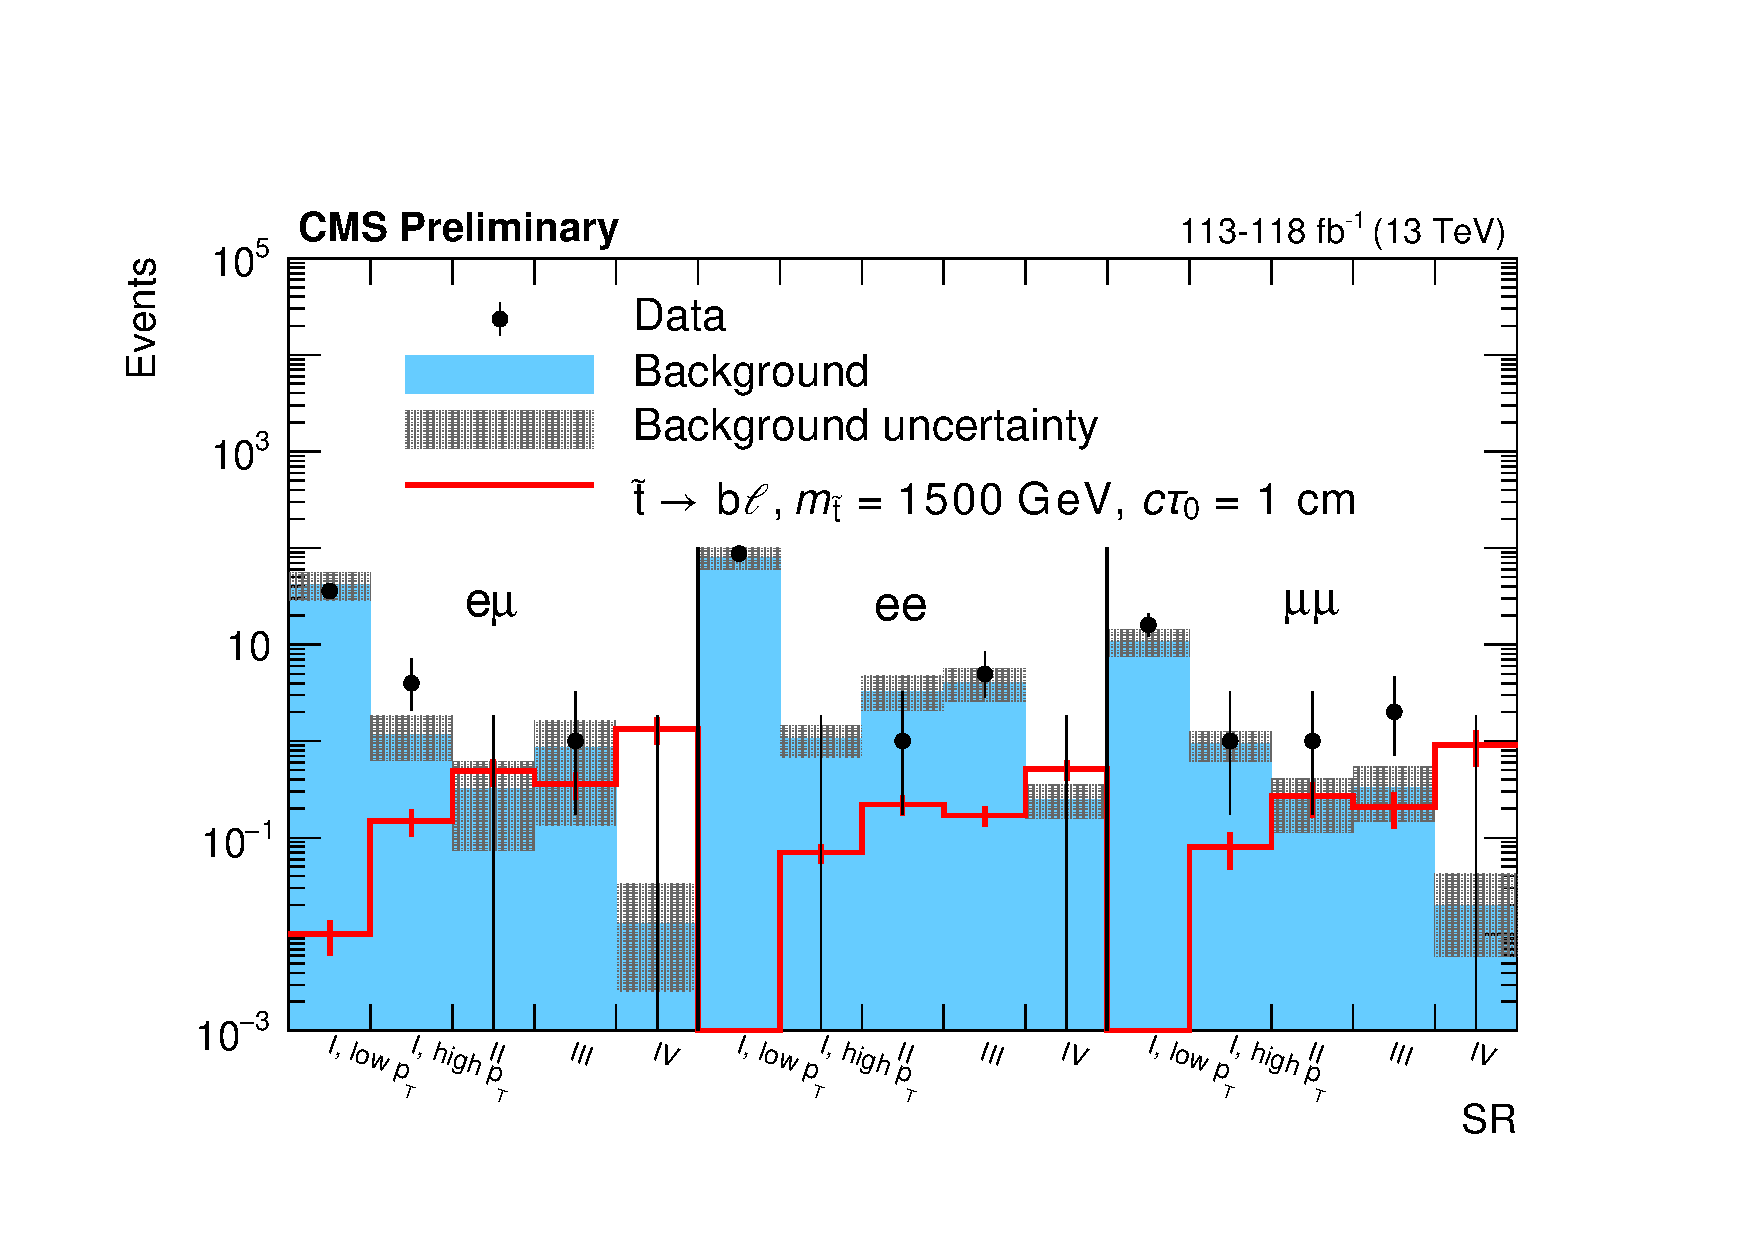
\includegraphics[width=\textwidth]{figures/results/SRRun2yields_CMSPreliminary.pdf}
\caption{The number of estimated background and observed events in each channel and SR, with a representative signal overlaid, for 2016--2018. For each background estimate and signal yield, the total uncertainty is given. Statistical uncertainties are given on observed yields.}
\label{yields_combined}
\end{figure}

Figure~\ref{d0_d0_data} shows two-dimensional \ad distributions of data events that pass the preselection, and Fig.~\ref{d0_d0_sr_data} shows the same but for data events in the inclusive SR. Figure~\ref{d0_d0_sr_data_and_signal} shows the same along with a representative signal point.

\begin{figure}
\centering
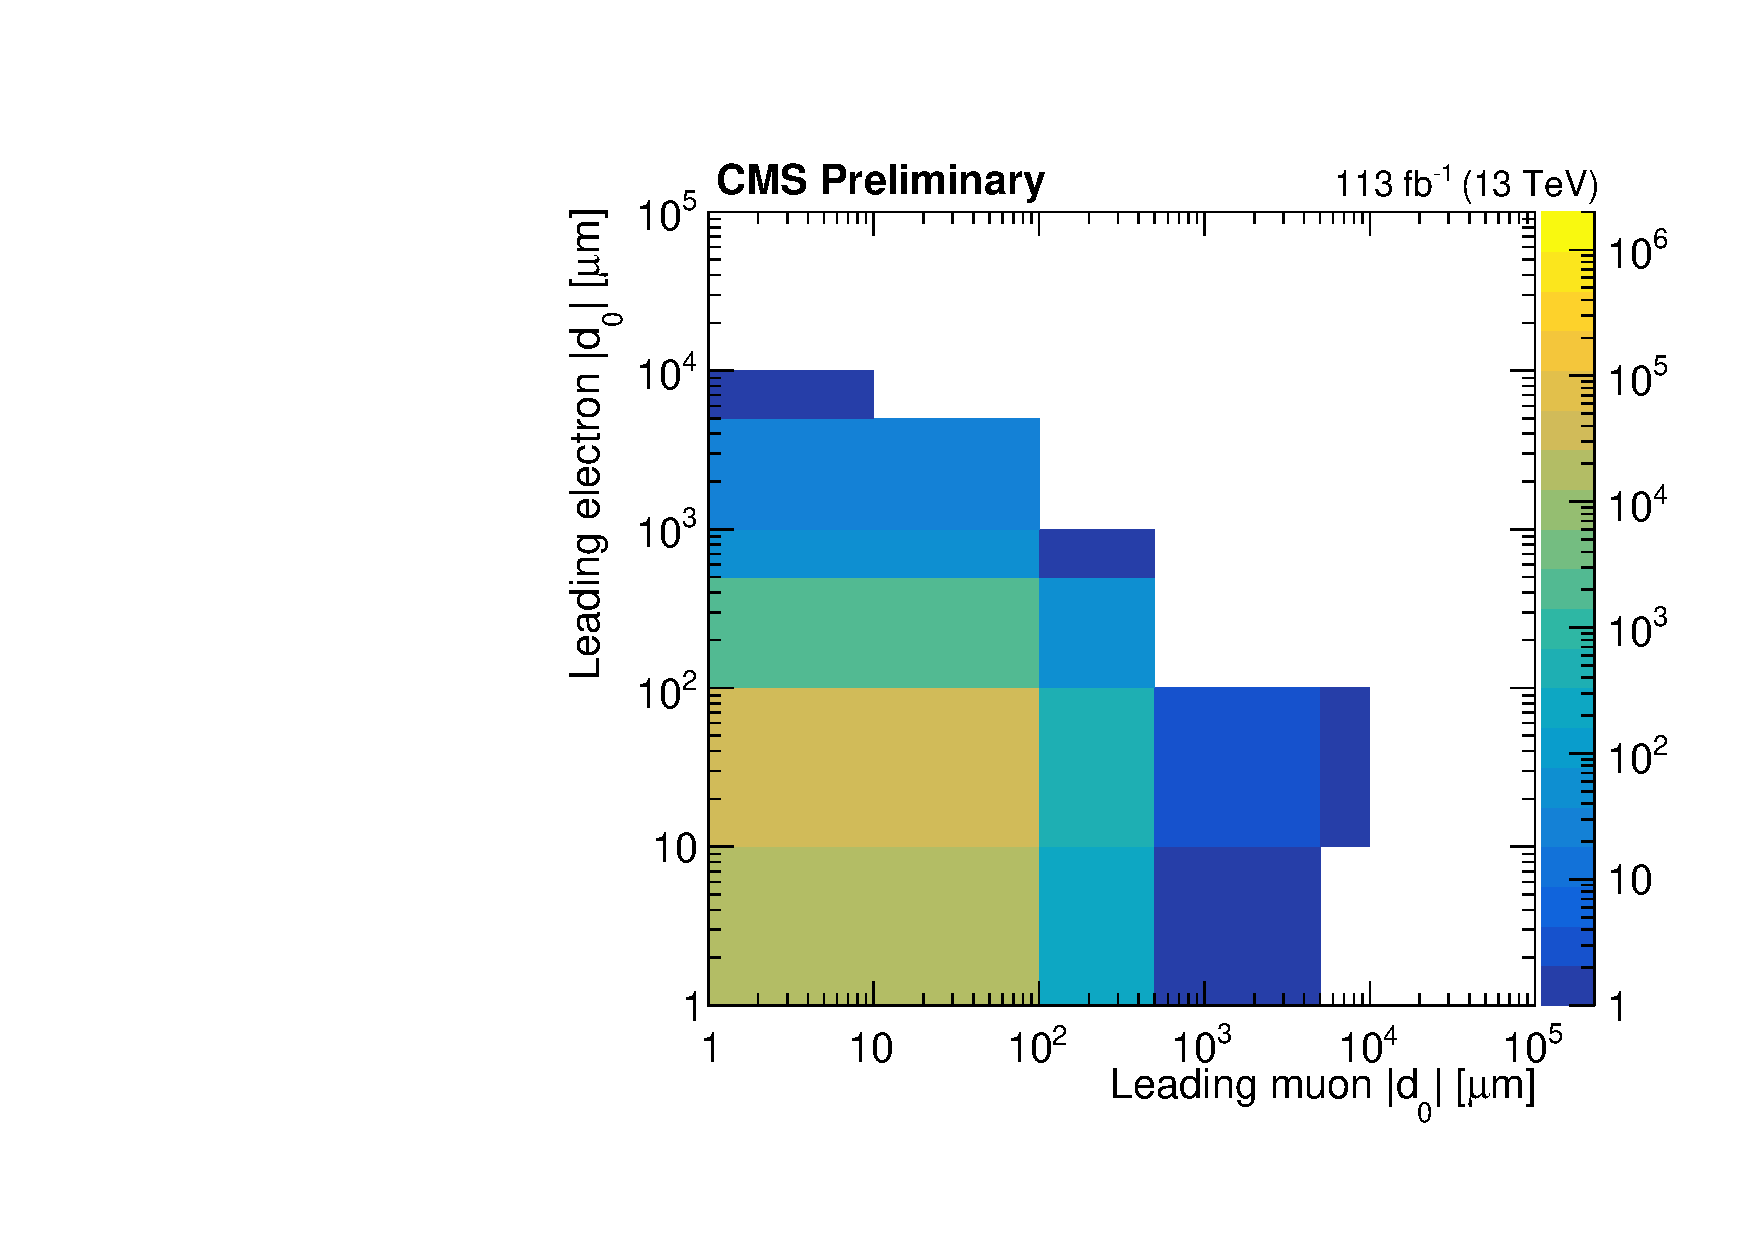
\includegraphics[width=0.32\textwidth]{figures/results/d0vsd0_emu_CMSPreliminary.pdf}
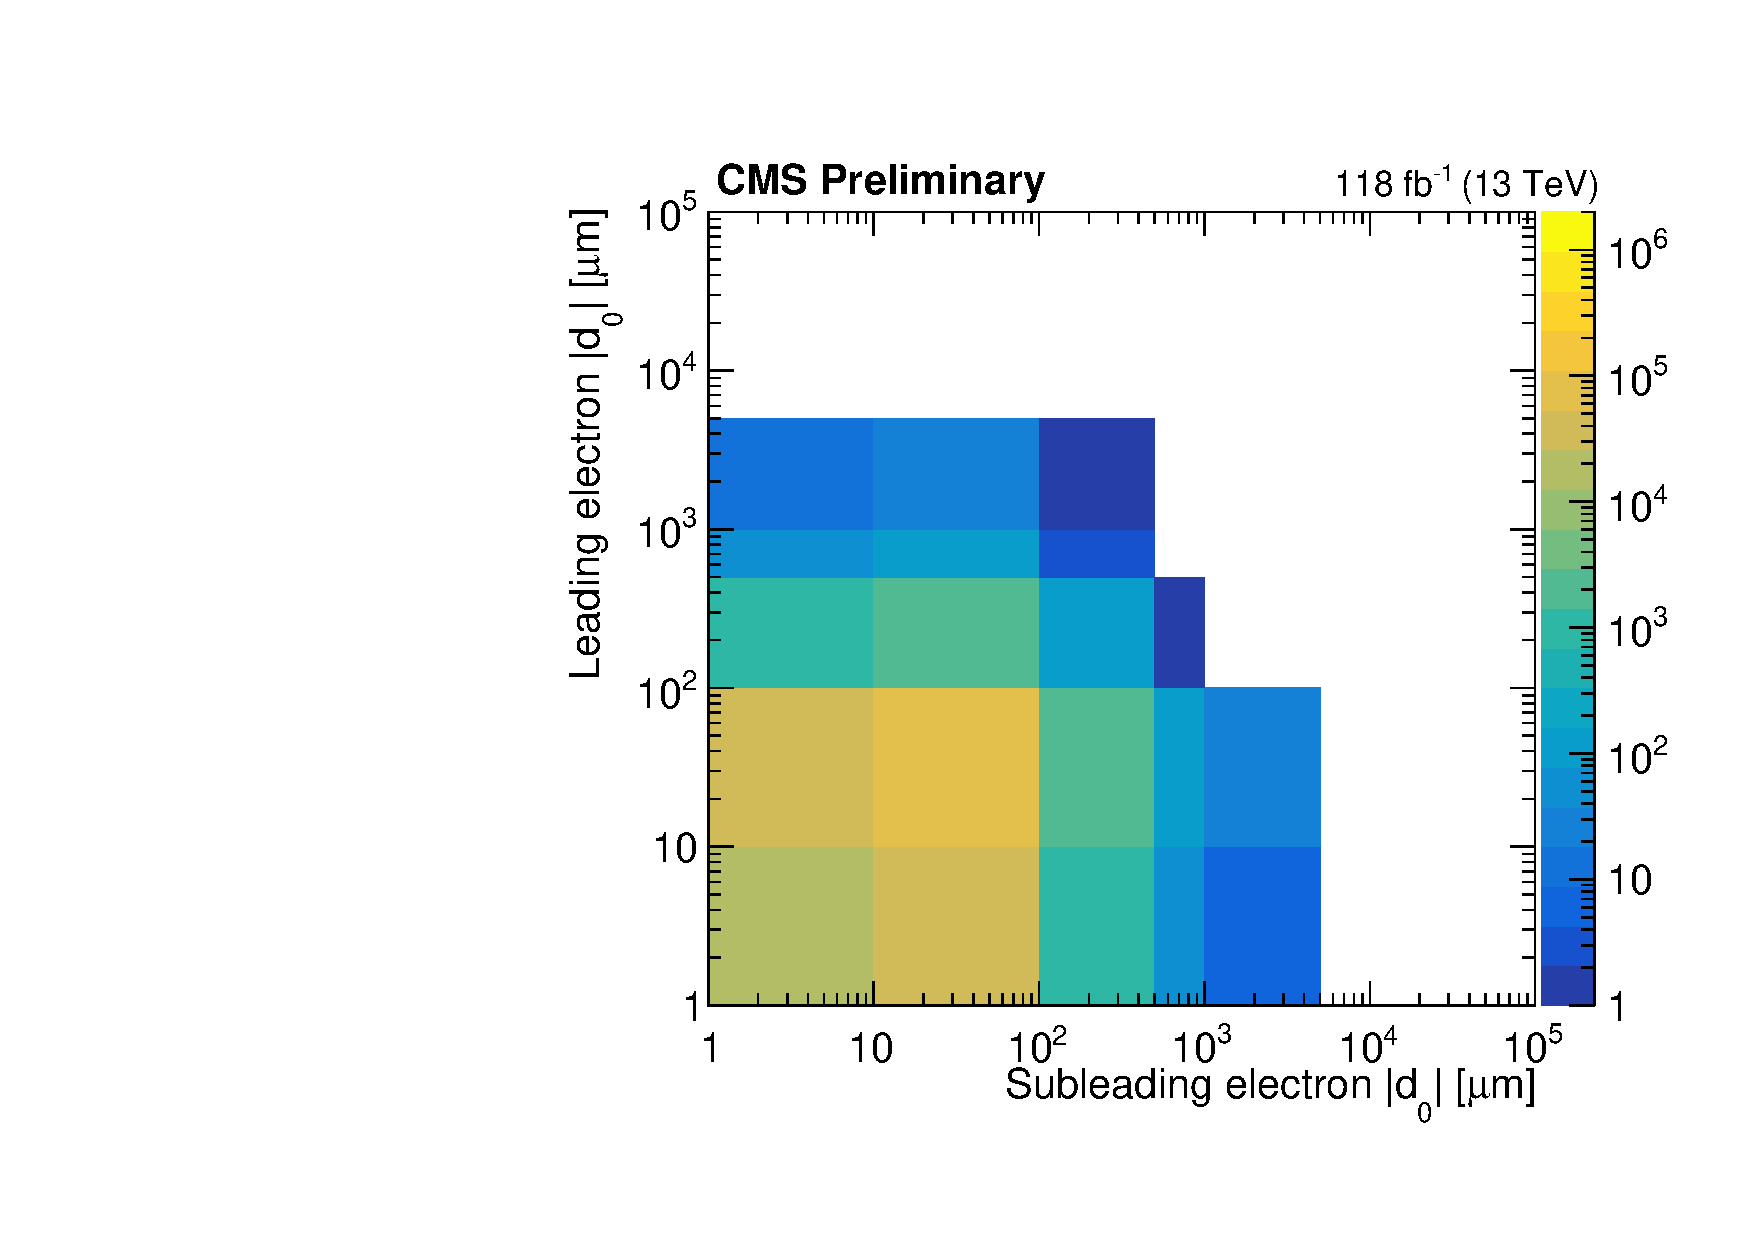
\includegraphics[width=0.32\textwidth]{figures/results/d0vsd0_ee_CMSPreliminary.pdf}
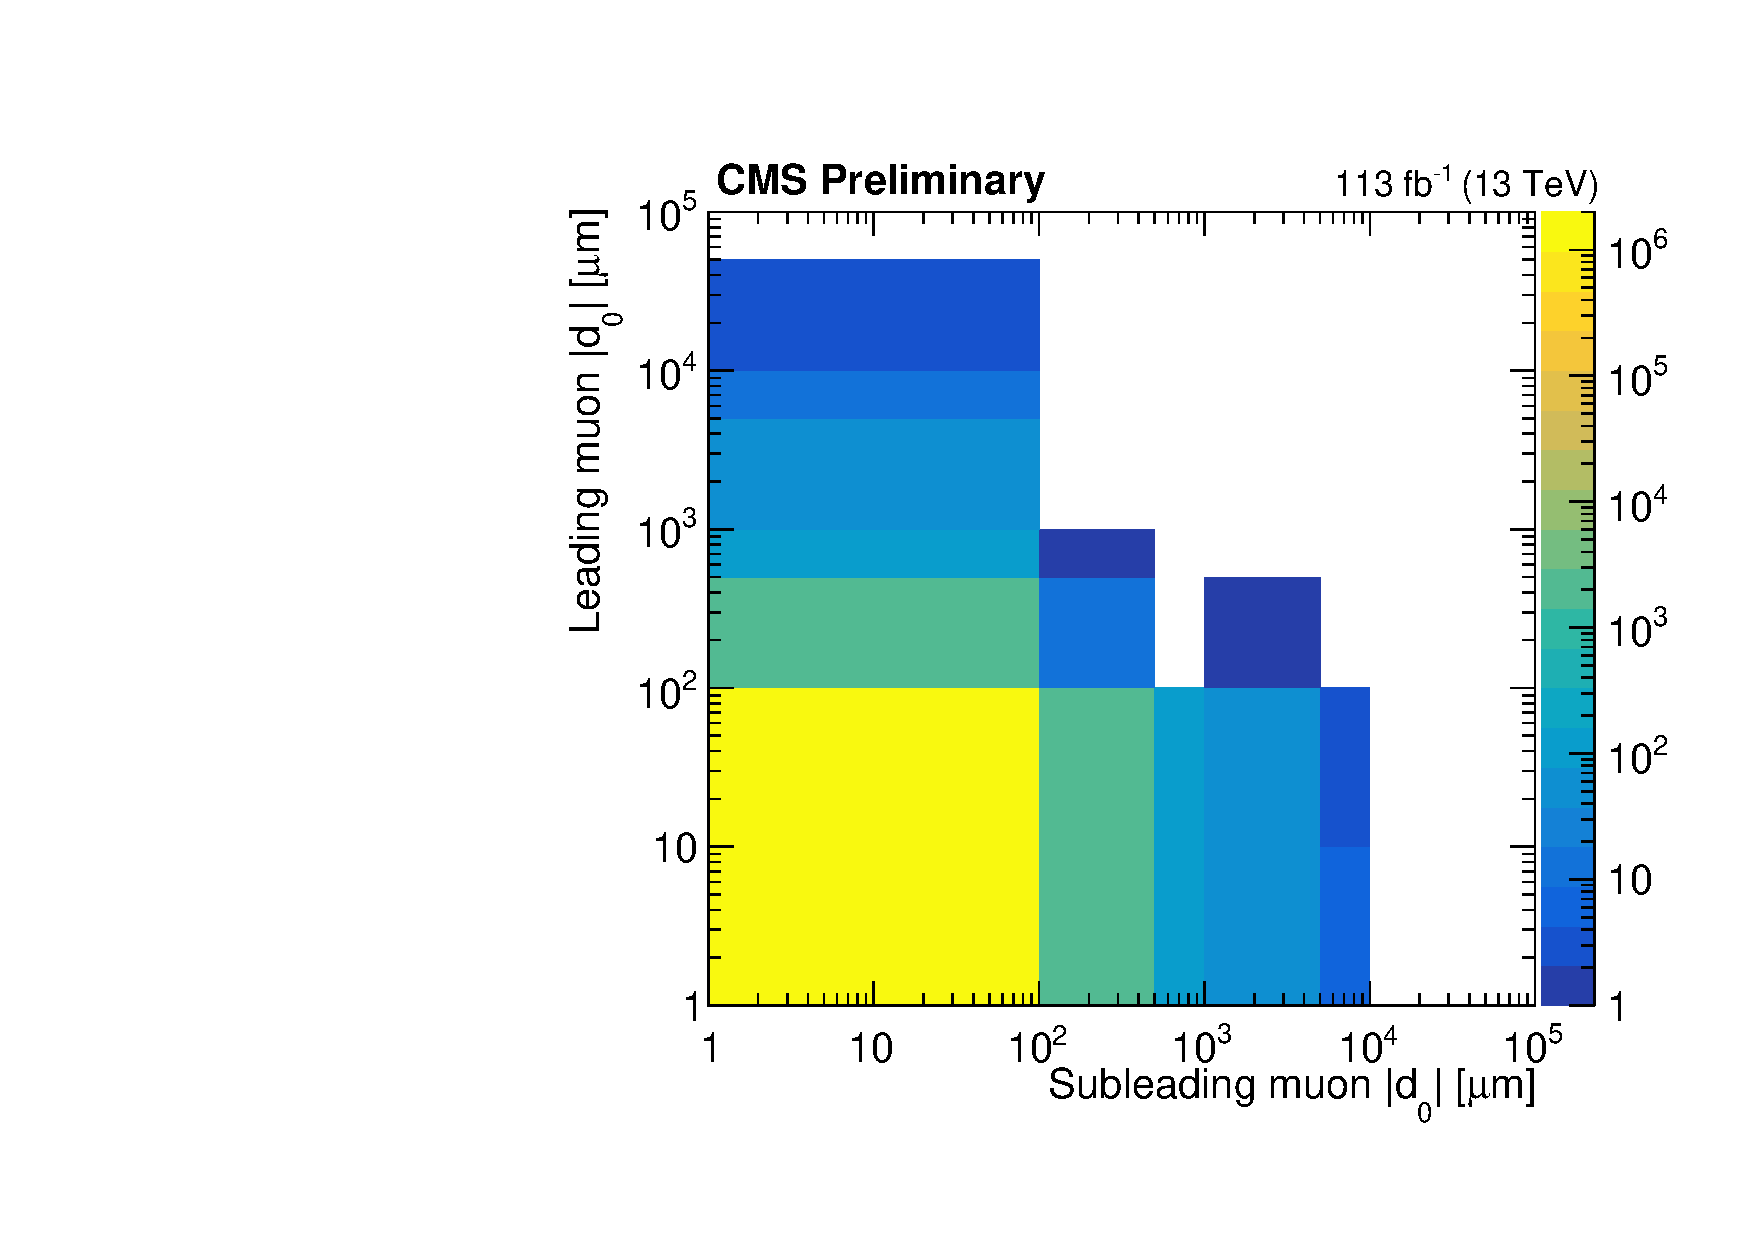
\includegraphics[width=0.32\textwidth]{figures/results/d0vsd0_mumu_CMSPreliminary.pdf}
\caption{
Two-dimensional distributions of \ada and \adb, for the events in data that pass the $\Pe\Pgm$ (left), $\Pe\Pe$ (middle), and $\Pgm\Pgm$ (right) preselection. The bins along the x and y axes contain underflow. The inclusive signal region covers the region between \SI{100}{\um} and \SI{10}{\cm} in each \ad variable shown.
}
\label{d0_d0_data}
\end{figure}

\begin{figure}
\centering
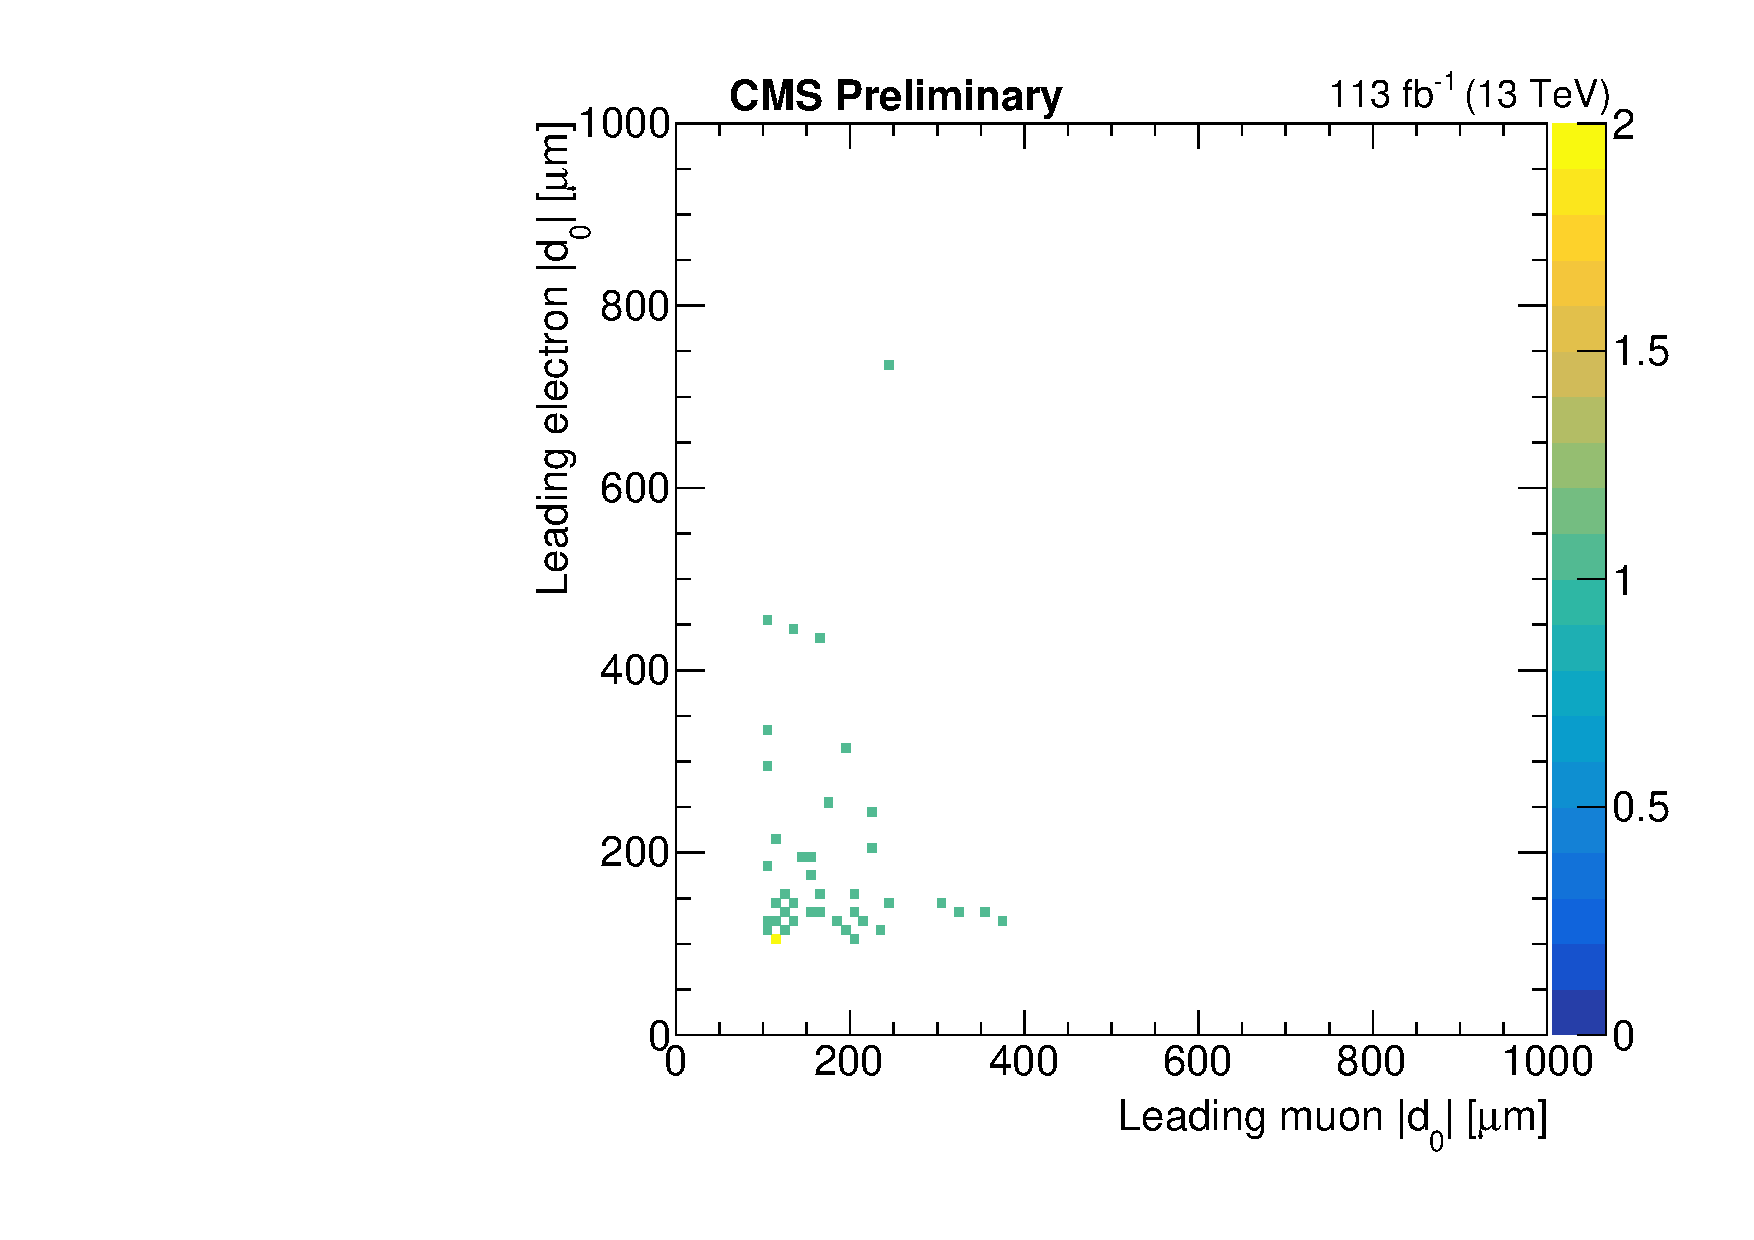
\includegraphics[width=0.31\textwidth]{figures/results/electronAbsD0[0]_vs_muonAbsD0[0]_1000um.pdf}
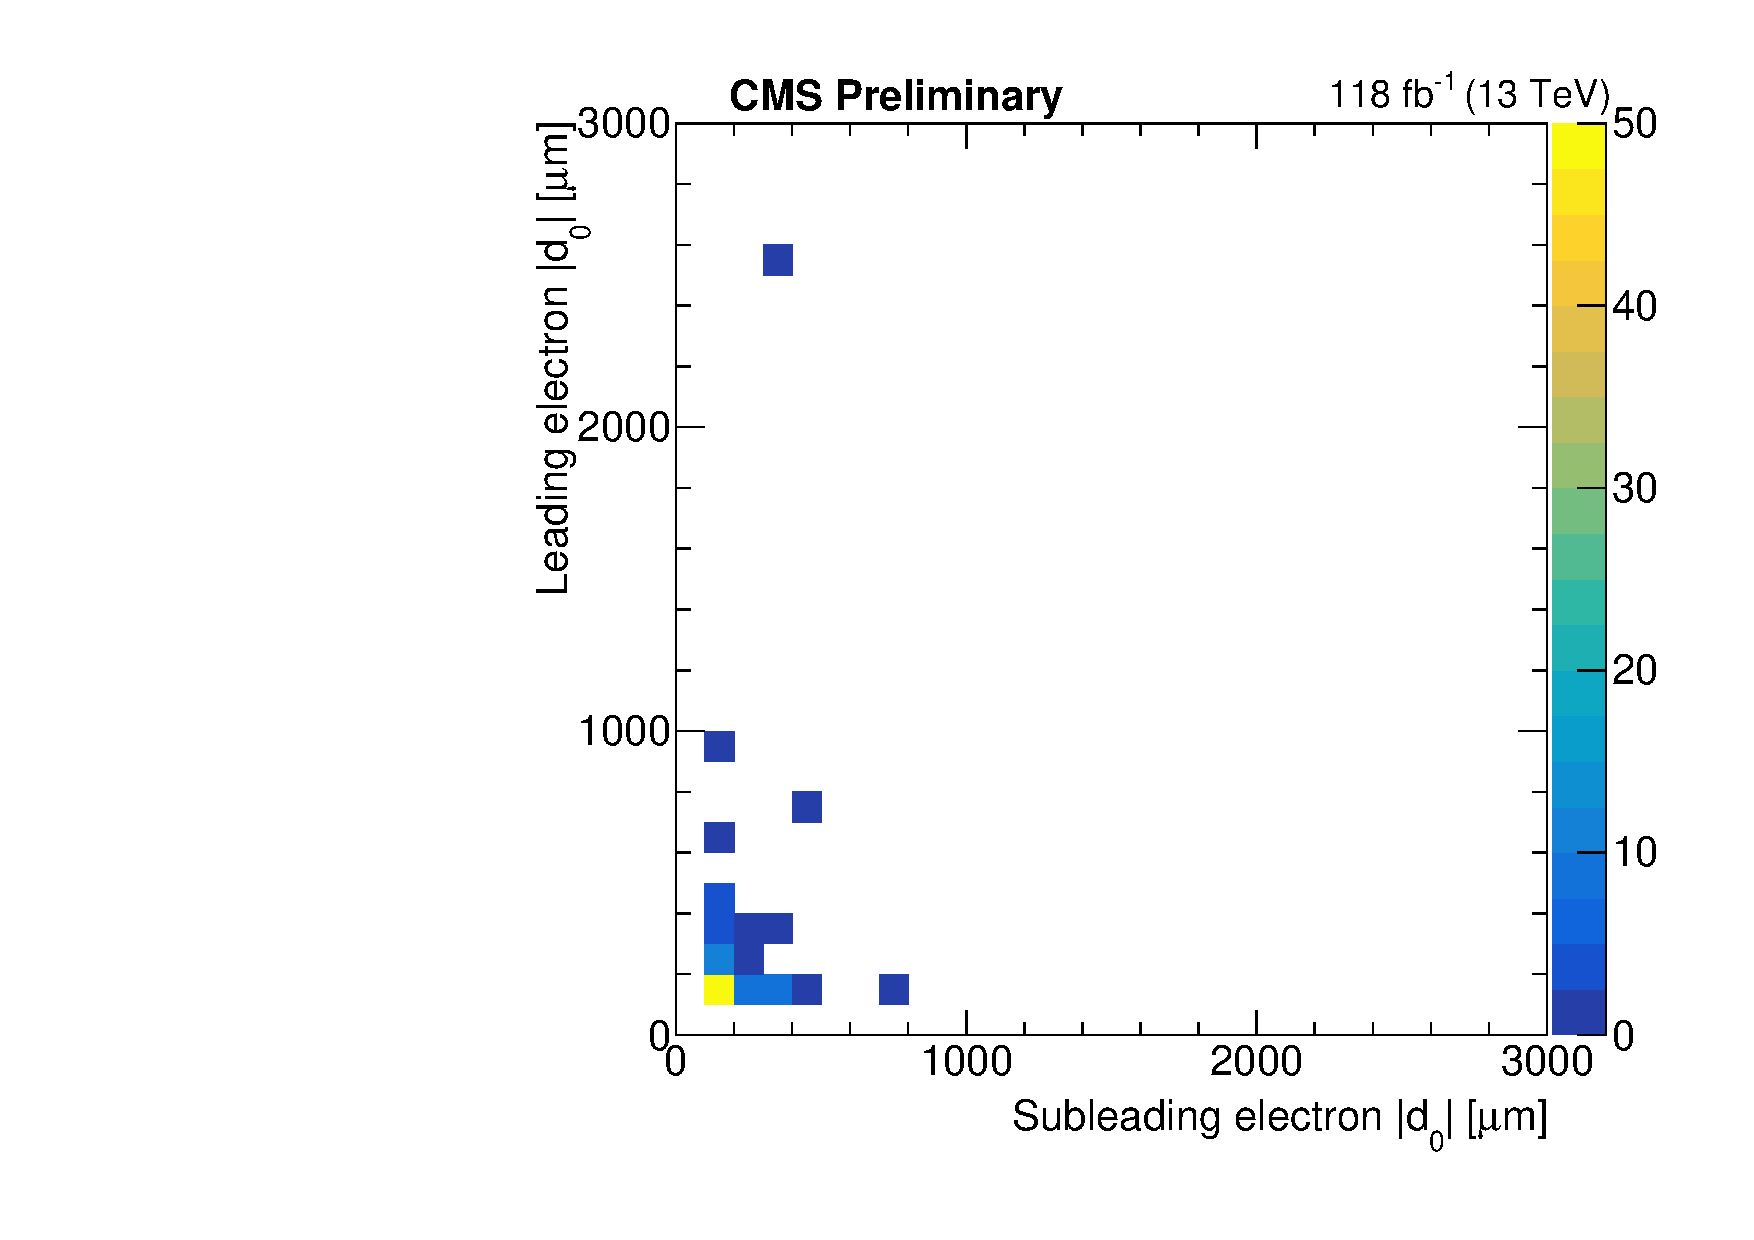
\includegraphics[width=0.31\textwidth]{figures/results/electronAbsD0[0]_vs_electronAbsD0[1]_10000um.pdf}
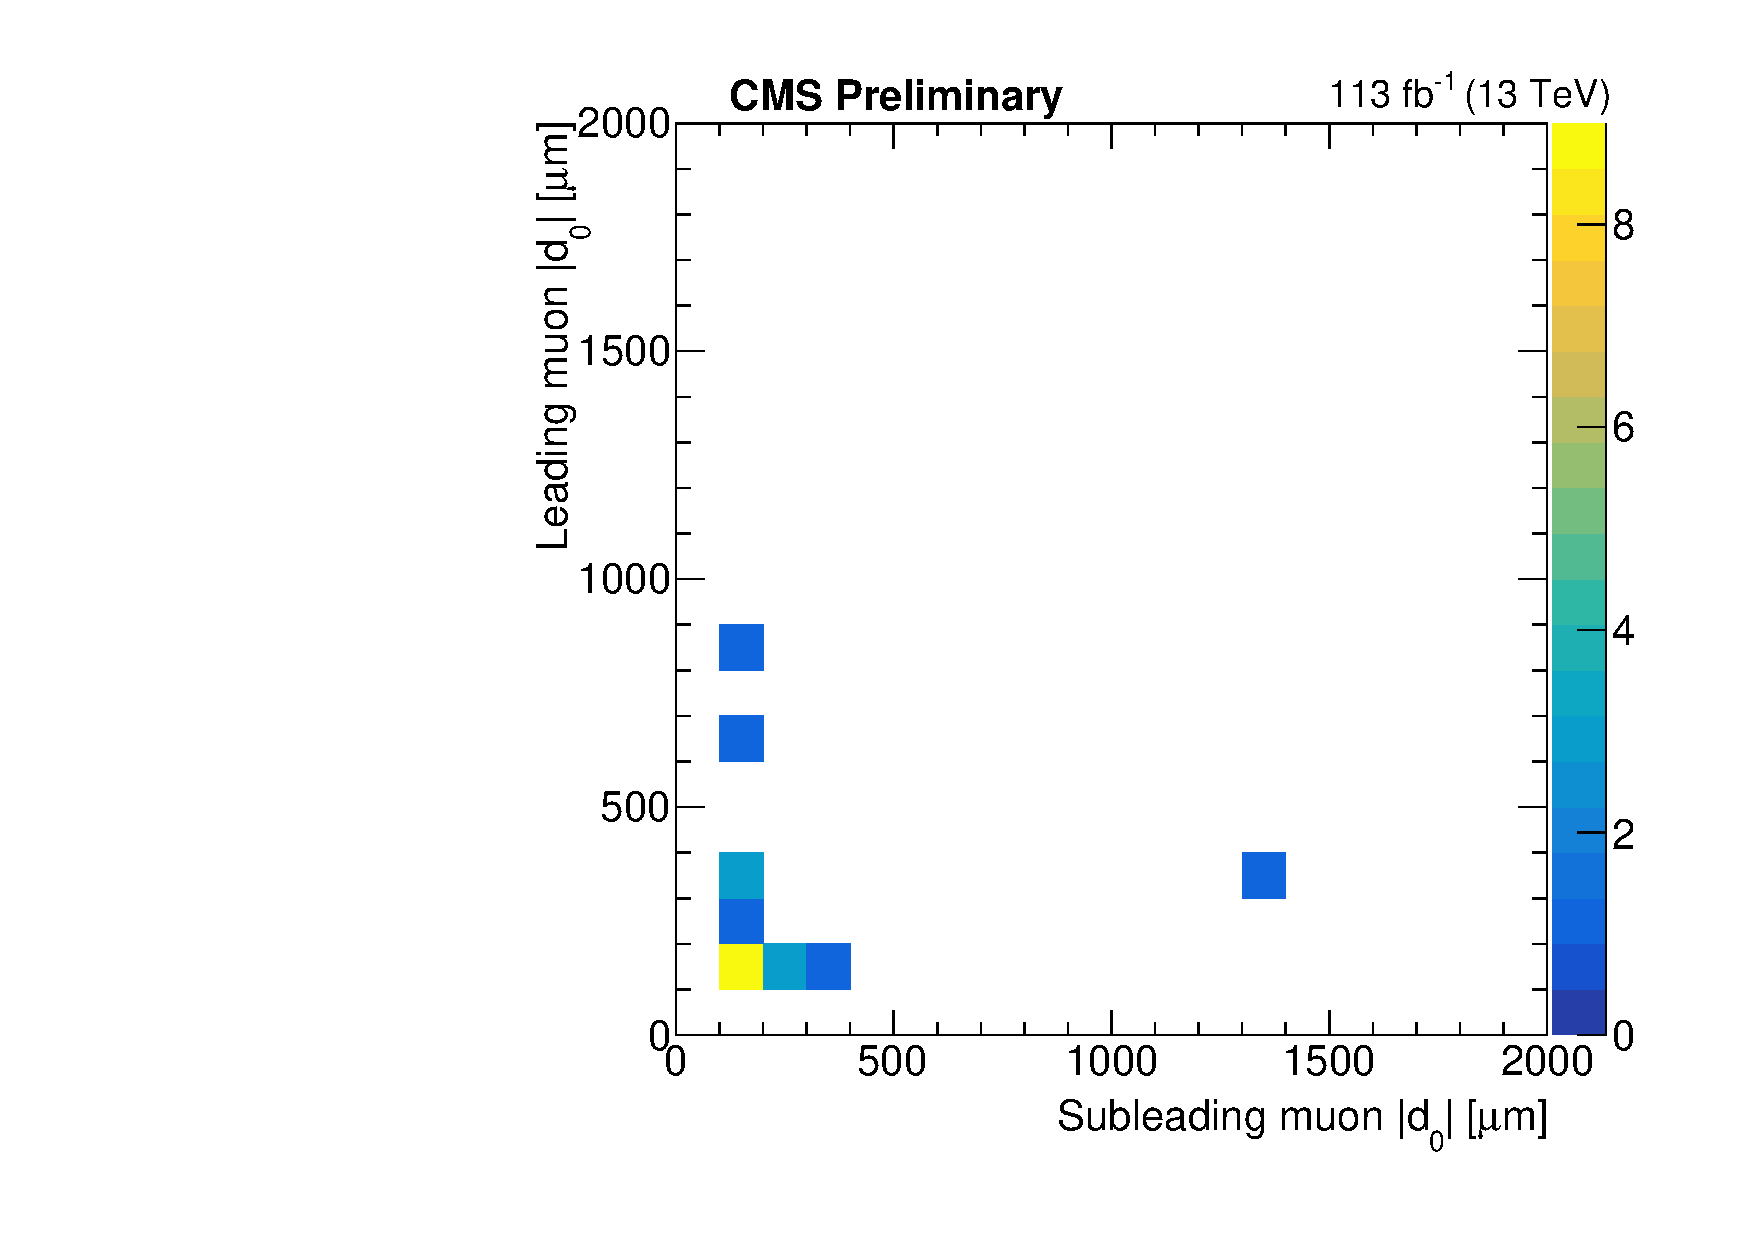
\includegraphics[width=0.31\textwidth]{figures/results/muonAbsD0[0]_vs_muonAbsD0[1]_10000um.pdf}
\caption{
Two-dimensional distributions of \ada and \adb, for data events in the inclusive SR in the $\Pe\Pgm$ (left), $\Pe\Pe$ (middle), and $\Pgm\Pgm$ (right) channels.
}
\label{d0_d0_sr_data}
\end{figure}

\subsection{Observed events}
This section provides a summary of observations recorded while examining event displays of the signal region events.

In general, the SR events appear to be SM events from the proton-proton collision. Specifically, we see no evidence of leptons from cosmic rays, material interactions, or signal.

In the $\Pe\Pgm$ channel, the SR events tend to have several jets and often have significant \ptmiss. Many events have muon $\phi$ values such that the muon system hits are all near the edges of detector sections or muon $\eta$ values such that the muon is near the barrel/endcap transition in the muon system. There are also a few events in which the electron and/or muon are associated with a different primary vertex than their associated track.

In the $\Pe\Pe$ channel, the majority of SR events contain at least one electron with $\abs{eta} > 1.1$, which increases the probability that their $d_0$ is poorly measured. Across all three years, most events fall into one of three categories: 
\begin{enumerate}
    \item Events with two electrons that appear to be from a boosted $Z$ boson, with an invariant mass between \num{80} and \SI{100}{\GeV}, opposite one or two jets
    \item Events with two electrons approximately back-to-back in $\phi$ with an invariant mass greater than \SI{100}{\GeV} and \ptmiss usually between \num{10} and \SI{40}{\GeV}
    \item Events that are similar to type 2 but with at least one jet and frequently \ptmiss between \num{70} and \SI{110}{\GeV}
\end{enumerate}

In the $\Pgm\Pgm$ channel, many events have an invariant mass consistent with the mass of the $Z$ boson and \ptmiss less than about \SI{60}{\GeV}. Most of the events found in 2017 and 2018 have an invariant mass higher than than the $Z$ boson mass and could be \ttbar events. Eight of the sixteen SR events in 2016 have two muons with $\phi$ values of about $\pm\pi/2$. All of the muon pairs in these eight events have an invariant mass consistent with a $Z$ boson. Furthermore, the $\cos(\alpha)$ and timing distributions of these muons imply that they are not from cosmic rays. Thirteen of the sixteen muons in these eight events have only one valid pixel hit, and event displays of these events show that the muon track often passes between or at the edge of pixel modules near the place where the two halves of the pixel detector barrel are joined. We believe that this feature causes the muon $d_0$ values to be poorly measured. \fxnote{probably add some event displays}

\subsection{Limits}

The data show no significant excess over background, so we set upper limits on the product of the signal production cross section ($\sigma$) and branching fraction ($\mathcal{B}$) using the HybridNew statistical method of the ``Combine'' tool developed by the CMS Higgs working group \cite{Junk_CLS,Read_CLS,Cowan:2010js,CMS-NOTE-2011-005}. The ABCD estimate is performed in Combine, which has the advantage that any signal contamination in the control regions is automatically accounted for. We perform a simultaneous counting experiment in each signal region bin. Figure~\ref{limits_individual} shows the 95\% confidence level ($\CL$) upper limits on the top squark mass as a function of its lifetime.
\fxnote{top squark, Higgs boson, and slepton lifetimes as a function of their masses, for each of the three channels.}

The variation in the size and shape of the exclusion regions between the three channels is mostly explained by variation in signal yields between the three channels. Looking at the high-\pt bin of SR I, which is the most sensitive bin for top squarks with large masses and small lifetimes, we find that the simulated signal yield is highest in the $\Pe\Pgm$. This difference between the $\Pe\Pgm$ and same-flavor channels is a result of simple combinatorics: the two independent top squark decays will result in an $\Pe\Pgm$ final state twice as often as an $\Pe\Pe$ or $\Pgm\Pgm$ final state. In this bin, the $\Pe\Pe$- and $\Pgm\Pgm$-channel signal yields are similar. SR IV drives the sensitivity for top squarks with large lifetimes. Because CMS identifies muons with higher efficiency than it does electrons, the $\Pgm\Pgm$ channel has the largest simulated signal yield in SR IV when considering top squarks with lifetimes $\gtrsim\SI{10}{\cm}$. For this same reason, the $\Pe\Pe$ channel has the smallest signal yield out of the three channels in SR IV when considering top squark lifetimes $\gtrsim\SI{10}{\cm}$. Taking all of these effects together, we find that the $\Pe\Pgm$ channel is the most sensitive for lifetimes ${\lesssim}\SI{10}{\cm}$ while the $\Pgm\Pgm$ channel is the most sensitive for lifetimes ${\gtrsim}\SI{10}{\cm}$.

Figure~\ref{limits_combined} shows the 95\% $\CL$ upper limits for the combination of the three channels. The top squark limits assume $\mathcal{B}(\PSQt \to \cPqb \Pl)=\mathcal{B}(\PSQt \to \cPqd \Pl)=100\%$, and each $\Pl$ has an equal probability of being an electron, a muon, or a tau lepton.
\fxnote{The Higgs boson limits assume $\mathcal{B}(\PH \to \mathrm{S}\mathrm{S}=100\%$, and each $\Pl$ has an equal probability of being an electron or a muon. The slepton limits assume the superpartners of the left- and right-handed leptons are mass degenerate.}

\begin{figure}
\centering
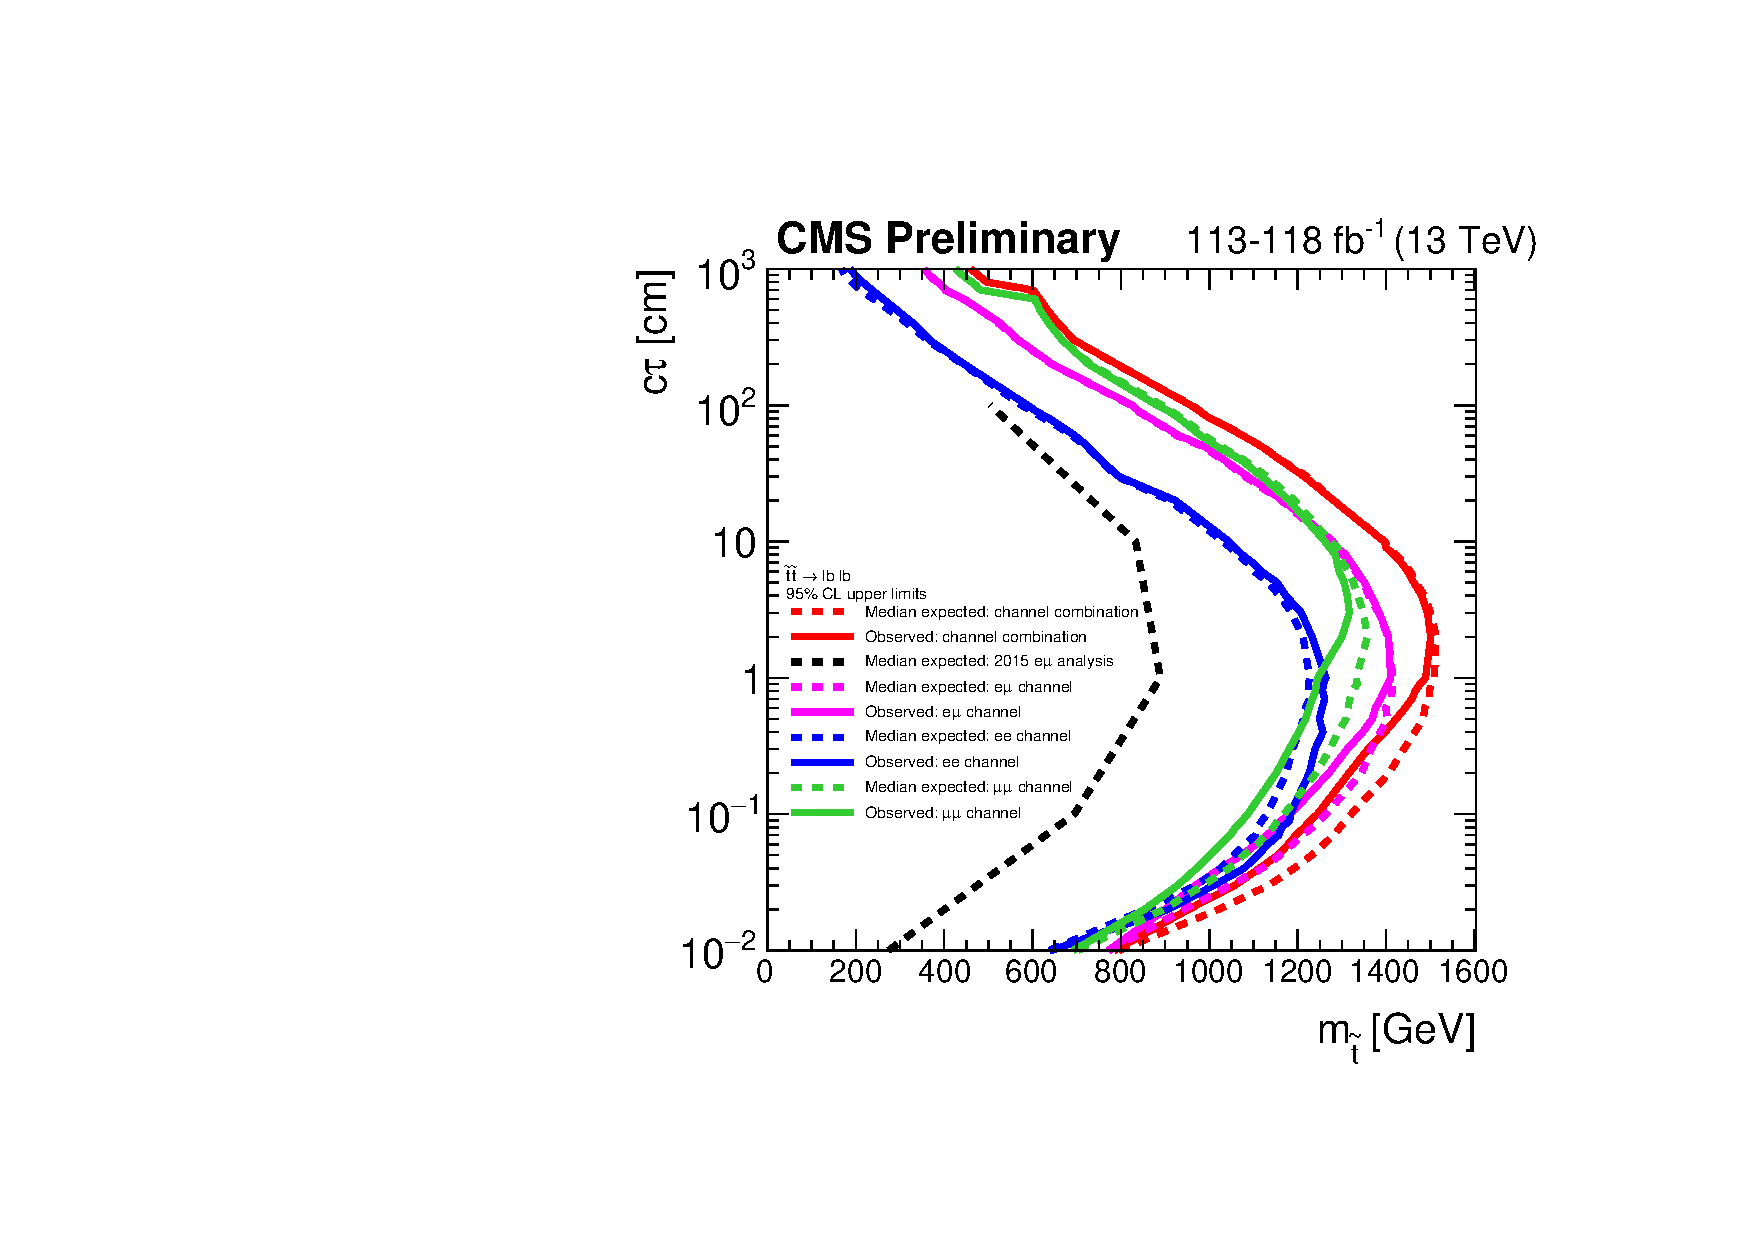
\includegraphics[width=0.65\textwidth]{figures/results/2DlimitsStopToLB.pdf}
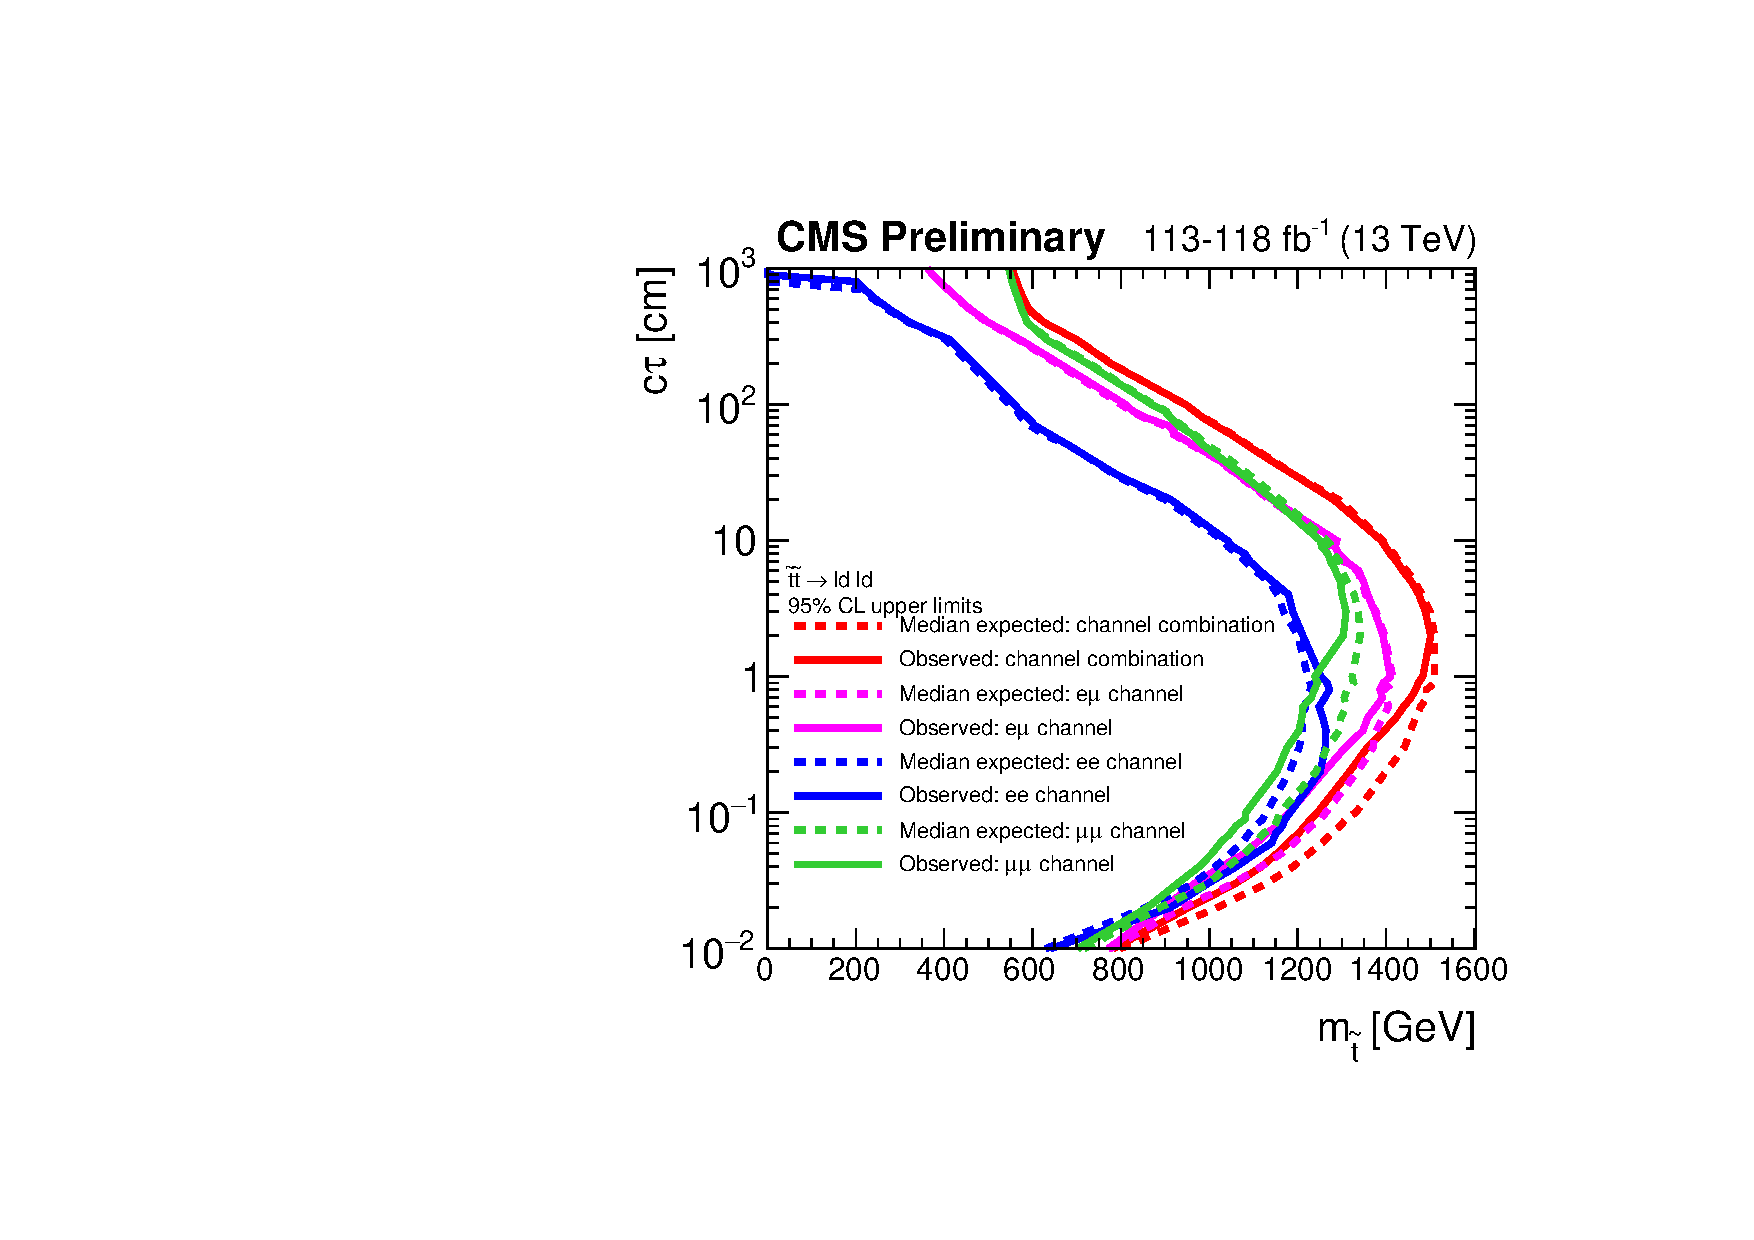
\includegraphics[width=0.65\textwidth]{figures/results/2DlimitsStopToLD.pdf}
\caption{The 95\% $\CL$ upper limits on the top squark mass ($m_{\PSQt}$) as a function of its lifetime ($c\tau$), for the $\Pe\Pgm$, $\Pe\Pe$, and $\Pgm\Pgm$ channels. The \stoptolb (top) and \stoptold (bottom) processes are shown.} 
%The $\PSQt\PASQt \to \PAl\PQb\:\Pl\PAQb $ (upper left), $\PSQt\PASQt \to \PAl\PQd\:\Pl\PAQd$ (upper right), $\PSl\PASl \to \PAl\PXXSG\:\Pl\PXXSG$ (lower left), and $\PH \to \PS\PS \to \Pl\PAl\:\Pl\PAl$ (lower right) processes are shown.}
\label{limits_individual}
\end{figure}

\begin{figure}
\centering
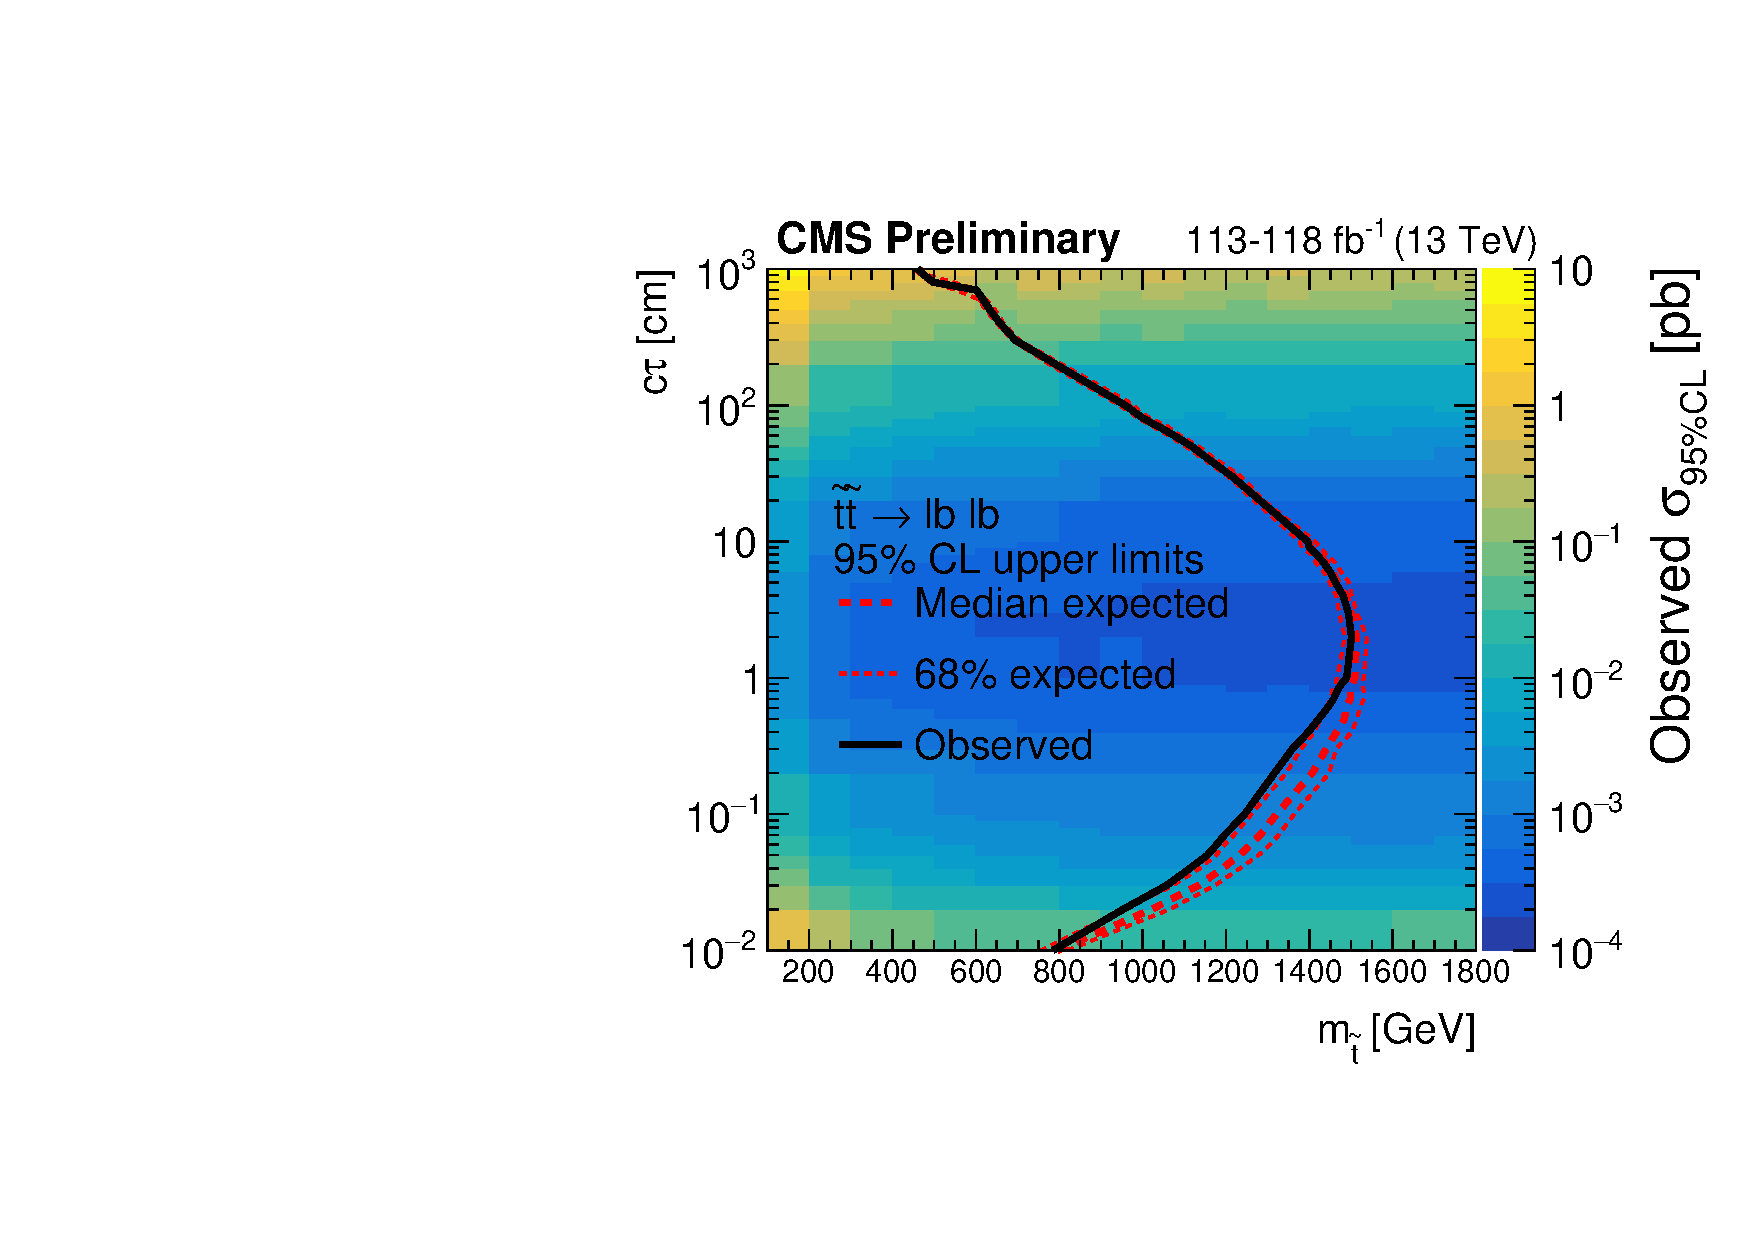
\includegraphics[width=0.65\textwidth]{figures/results/2DlimitsCombinedStopToLB.pdf}
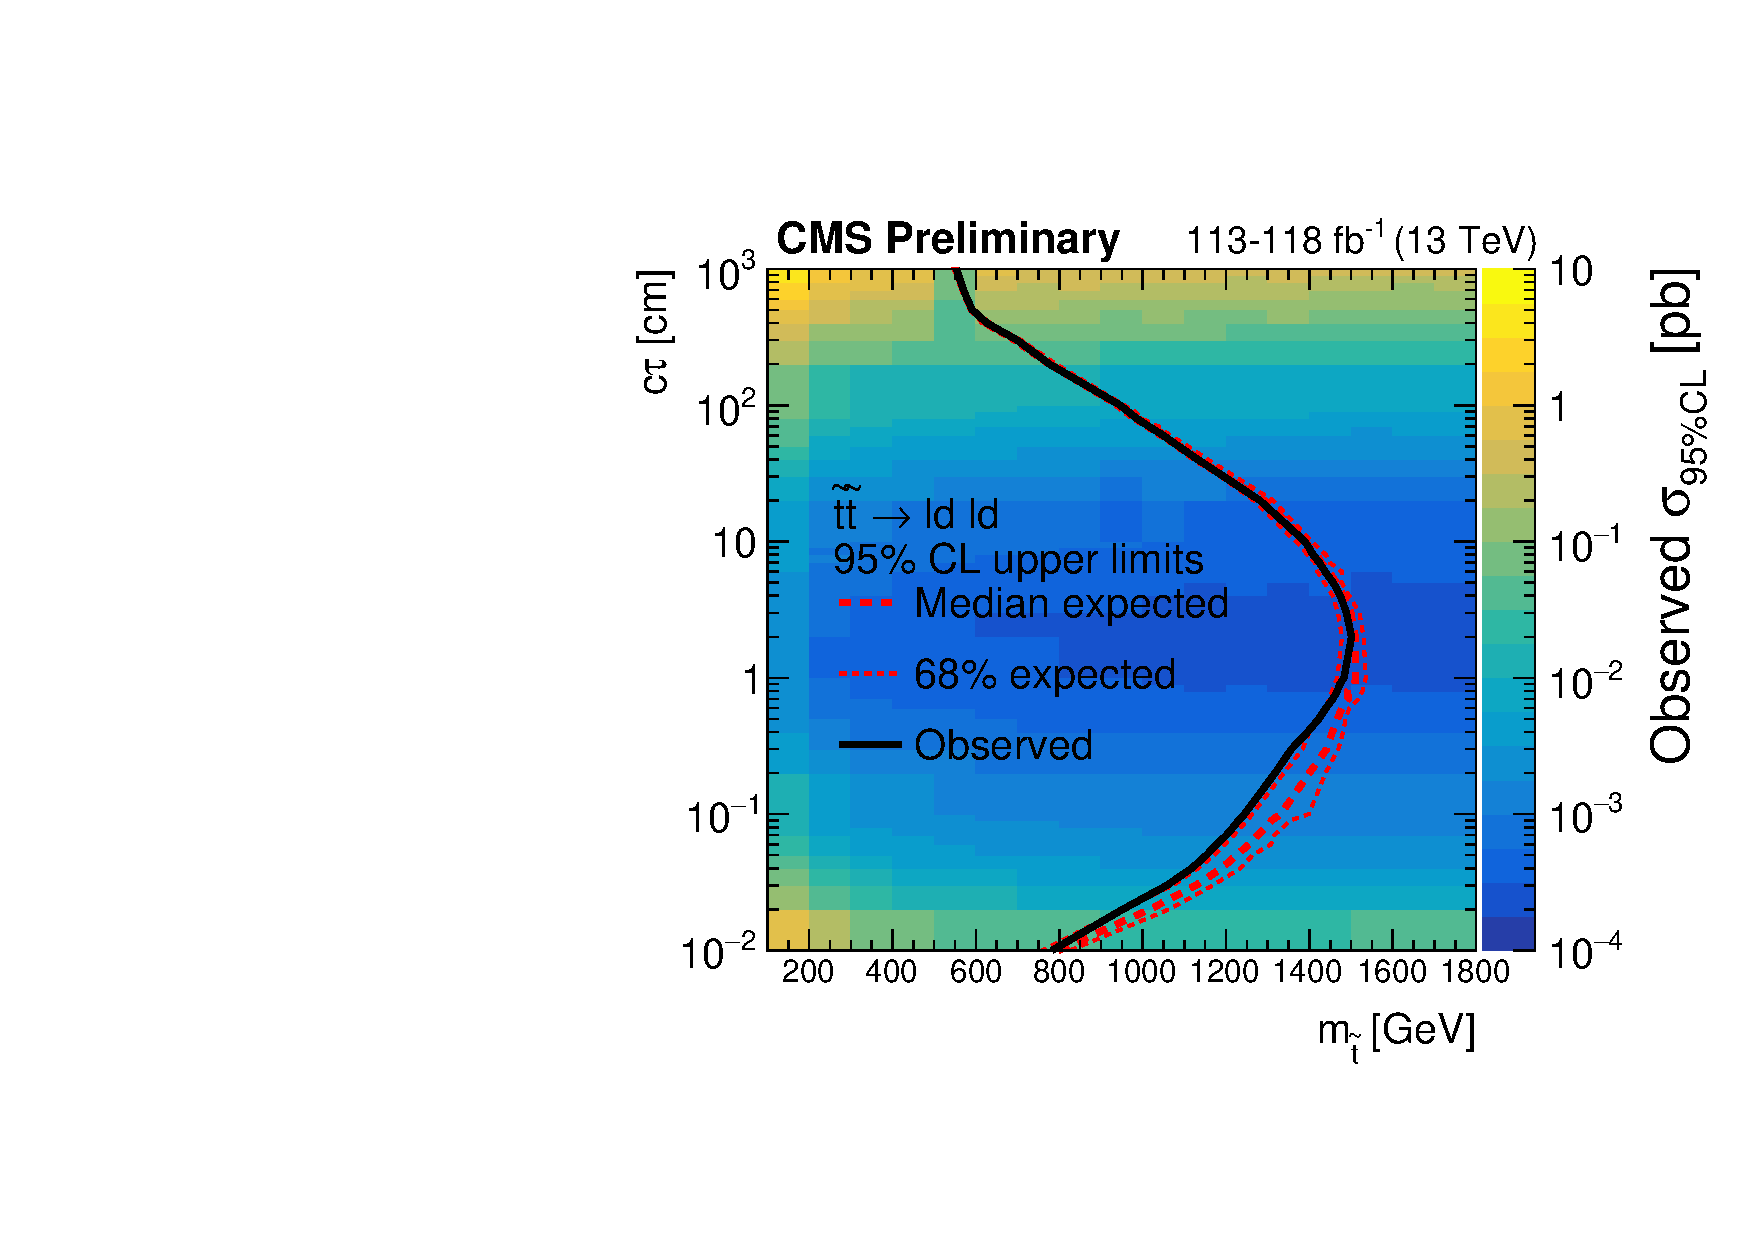
\includegraphics[width=0.65\textwidth]{figures/results/2DlimitsCombinedStopToLD.pdf}
\caption{The 95\% $\CL$ upper limits on the top squark mass ($m_{\PSQt}$) as a function of its lifetime ($c\tau$). The colors indicate the observed 95\% $\CL$ upper limit on the cross section. The \stoptolb (left) and \stoptold (right) processes are shown.} 
%The $\PSQt\PASQt \to \PAl\PQb\:\Pl\PAQb $ (upper left), $\PSQt\PASQt \to \PAl\PQd\:\Pl\PAQd$ (upper right), $\PSl\PASl \to \PAl\PXXSG\:\Pl\PXXSG$ (lower left), and $\PH \to \PS\PS \to \Pl\PAl\:\Pl\PAl$ (lower right) processes are shown.}
\label{limits_combined}
\end{figure}

\subsection{Additional likelihood tests}
We also perform several statistical tests to help assess the significance of the differences between the observed and predicted SR yields and to ensure that the likelihood is handling the observed yields in a reasonable way.

We first compare the best-fit background yields under the background-only hypothesis while masking the signal regions with the best-fit background yields under the signal+background hypothesis using the full information from all signal and control regions. For simplicity, we refer to the first quantity as the pre-fit prediction and the second as the post-fit prediction. Table~\ref{pre_postfit_predictions} lists the pre- and post-fit predictions for each channel and SR, and Fig.~\ref{pre_postfit_prediction_pulls} shows associated pull distribution. We find that the differences between the pre- and post-fit predictions are consistent with the variation one would expect from purely statistical effects.

\begin{table}
\renewcommand{\arraystretch}{1.3}
\noindent \centering{}
\topcaption{The pre- and post-fit predictions for each signal region bin.}
\label{pre_postfit_predictions}
\begin{tabular}{llllll}
\hline
 & SR I, & SR I,  &  &  & \\
 & low \pt & high \pt & SR II & SR III & SR IV \\
 & bin & bin &  & & \\
\hline
\textit{2016 $\Pe\Pgm$}\\
- pre-fit     & $3.8\pm3.9$  & $0.40\pm0.45$ & $0.09\pm0.11$ & $0.15\pm0.13$ & $0.003\pm0.003$\\
- post-fit     & $7.1\pm2.0$  & $0.76\pm0.31$ & $0.08\pm0.08$ & $0.14\pm0.14$ & $0.003\pm0.003$\\

\textit{2017+2018 $\Pe\Pgm$}\\
- pre-fit      & $38\pm14$    & $0.75\pm0.40$ & $0.23\pm0.37$ & $0.71\pm0.90$ & $0.01\pm0.02$\\
- post-fit     & $31\pm5$     & $0.68\pm0.25$ & $0.20\pm0.17$ & $0.65\pm0.48$ & $0.01\pm0.01$\\

\textit{2016 $\Pe\Pe$}\\
- pre-fit      & $18\pm11$    & $0.22\pm0.17$ & $0.51\pm2.41$ & $0.43\pm2.06$ & $0.01\pm0.06$\\
- post-fit     & $35\pm5$     & $0.40\pm0.14$ & $0.50\pm0.75$ & $0.44\pm0.53$ & $0.01\pm0.02$\\

\textit{2017+2018 $\Pe\Pe$}\\
- pre-fit      & $62\pm17$    & $0.85\pm0.31$ & $2.8\pm0.9$   & $3.6\pm1.2$   & $0.25\pm0.09$\\
- post-fit     & $50\pm6$     & $0.65\pm0.19$ & $2.5\pm0.7$   & $3.2\pm0.9$   & $0.22\pm0.06$\\

\textit{2016 $\Pgm\Pgm$}\\
- pre-fit      & $7.4\pm3.3$  & $0.25\pm0.11$ & $0.17\pm0.11$ & $0.19\pm0.12$ & $0.01\pm0.01$\\
- post-fit     & $11\pm2$     & $0.37\pm0.10$ & $0.19\pm0.10$ & $0.21\pm0.12$ & $0.01\pm0.01$\\

\textit{2017+2018 $\Pgm\Pgm$}\\
- pre-fit      & $3.4\pm1.6$  & $0.69\pm0.32$ & $0.08\pm0.12$ & $0.14\pm0.18$ & $0.01\pm0.02$\\
- post-fit     & $2.5\pm1.1$  & $0.51\pm0.22$ & $0.14\pm0.36$ & $0.23\pm0.63$ & $0.02\pm0.05$\\
\hline
\end{tabular}
\end{table}
\begin{figure}[hbtp]
\centering
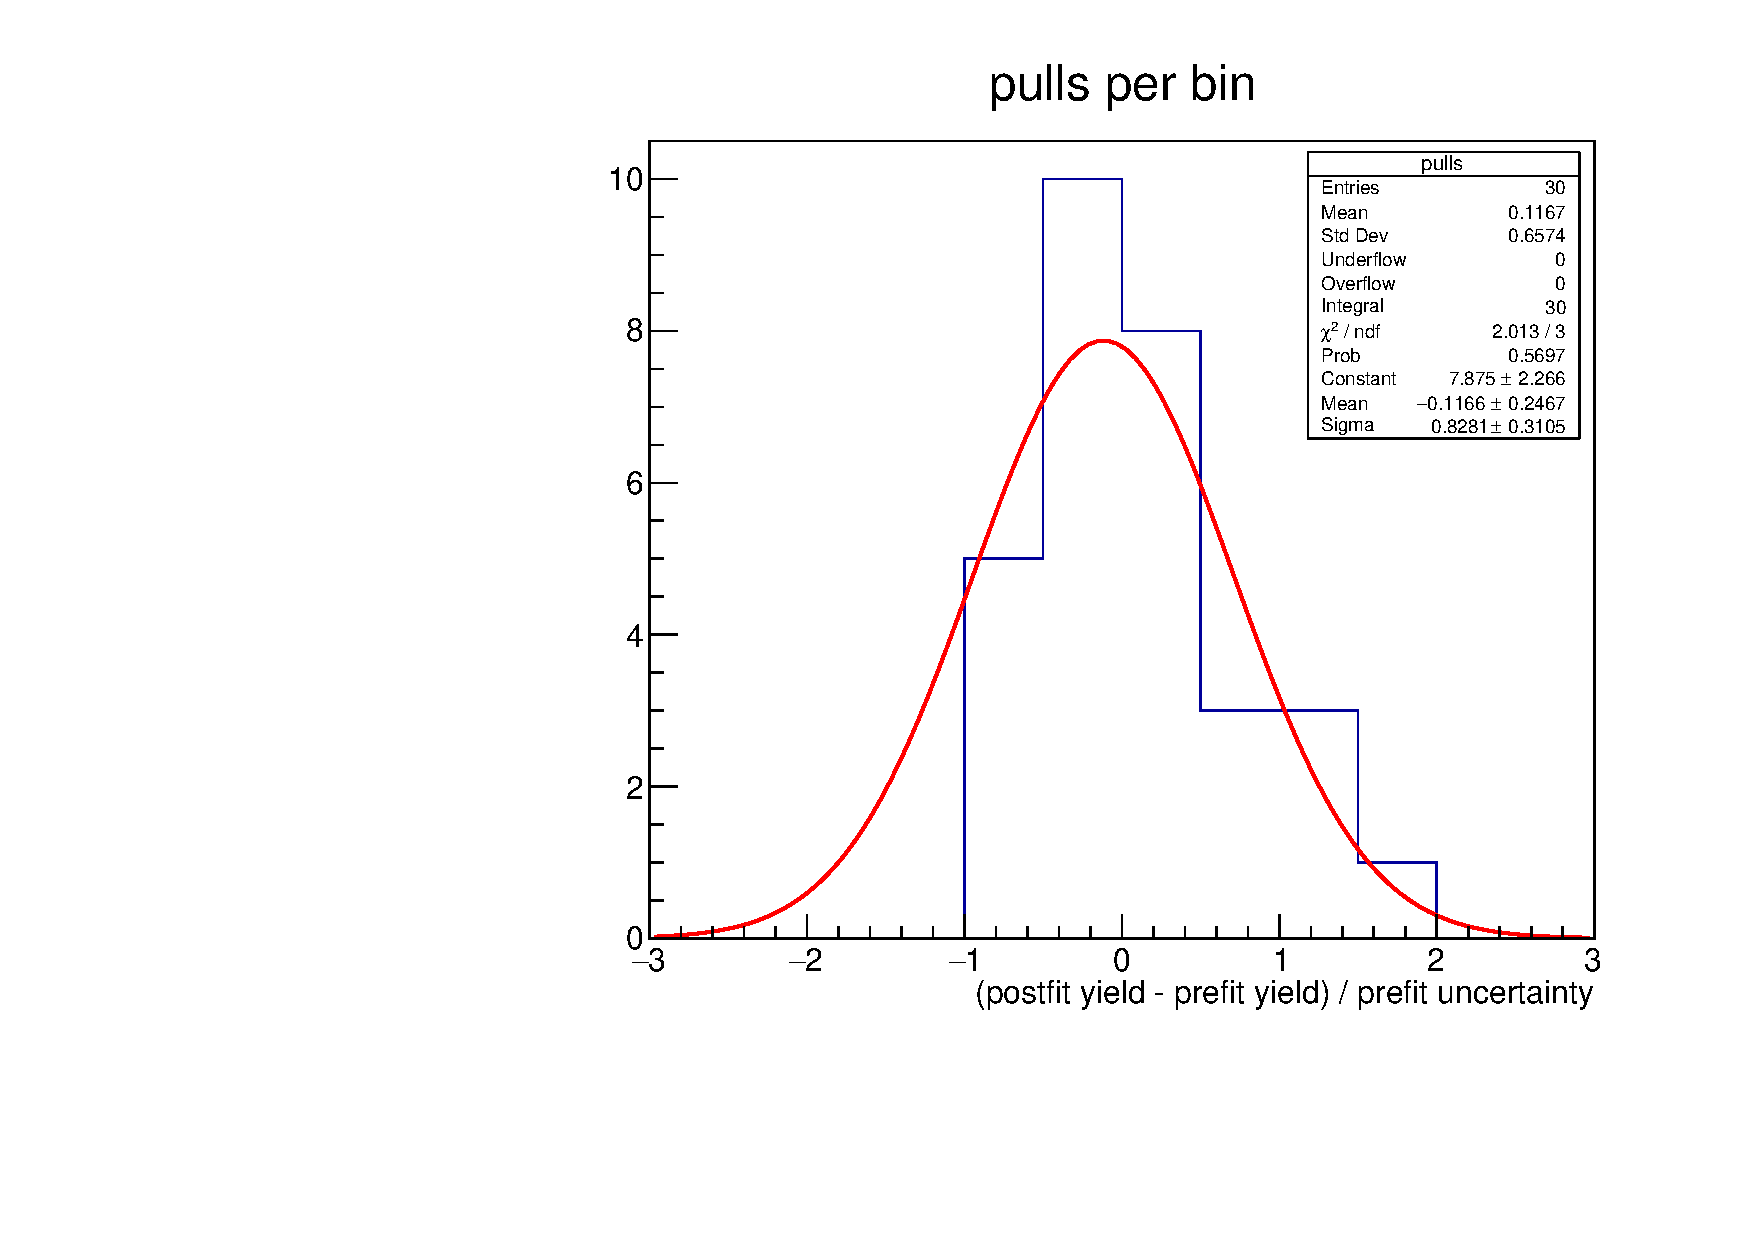
\includegraphics[scale=0.5]{figures/results/pullsPerBin.pdf}
\caption{The distribution of pulls for each signal region bin. Pulls are calculated as the difference between the post-fit background yield and the pre-fit background yield divided by the pre-fit background uncertainty.}
\label{pre_postfit_prediction_pulls}
\end{figure}

Next, we examine the equivalent pull distribution for background yield nuisance parameters. Figure~\ref{pre_postfit_param_pulls} shows that the differences in nuisance parameter values before and after the fit are also consistent with the variation one would expect from purely statistical effects.

\begin{figure}[hbtp]
\centering
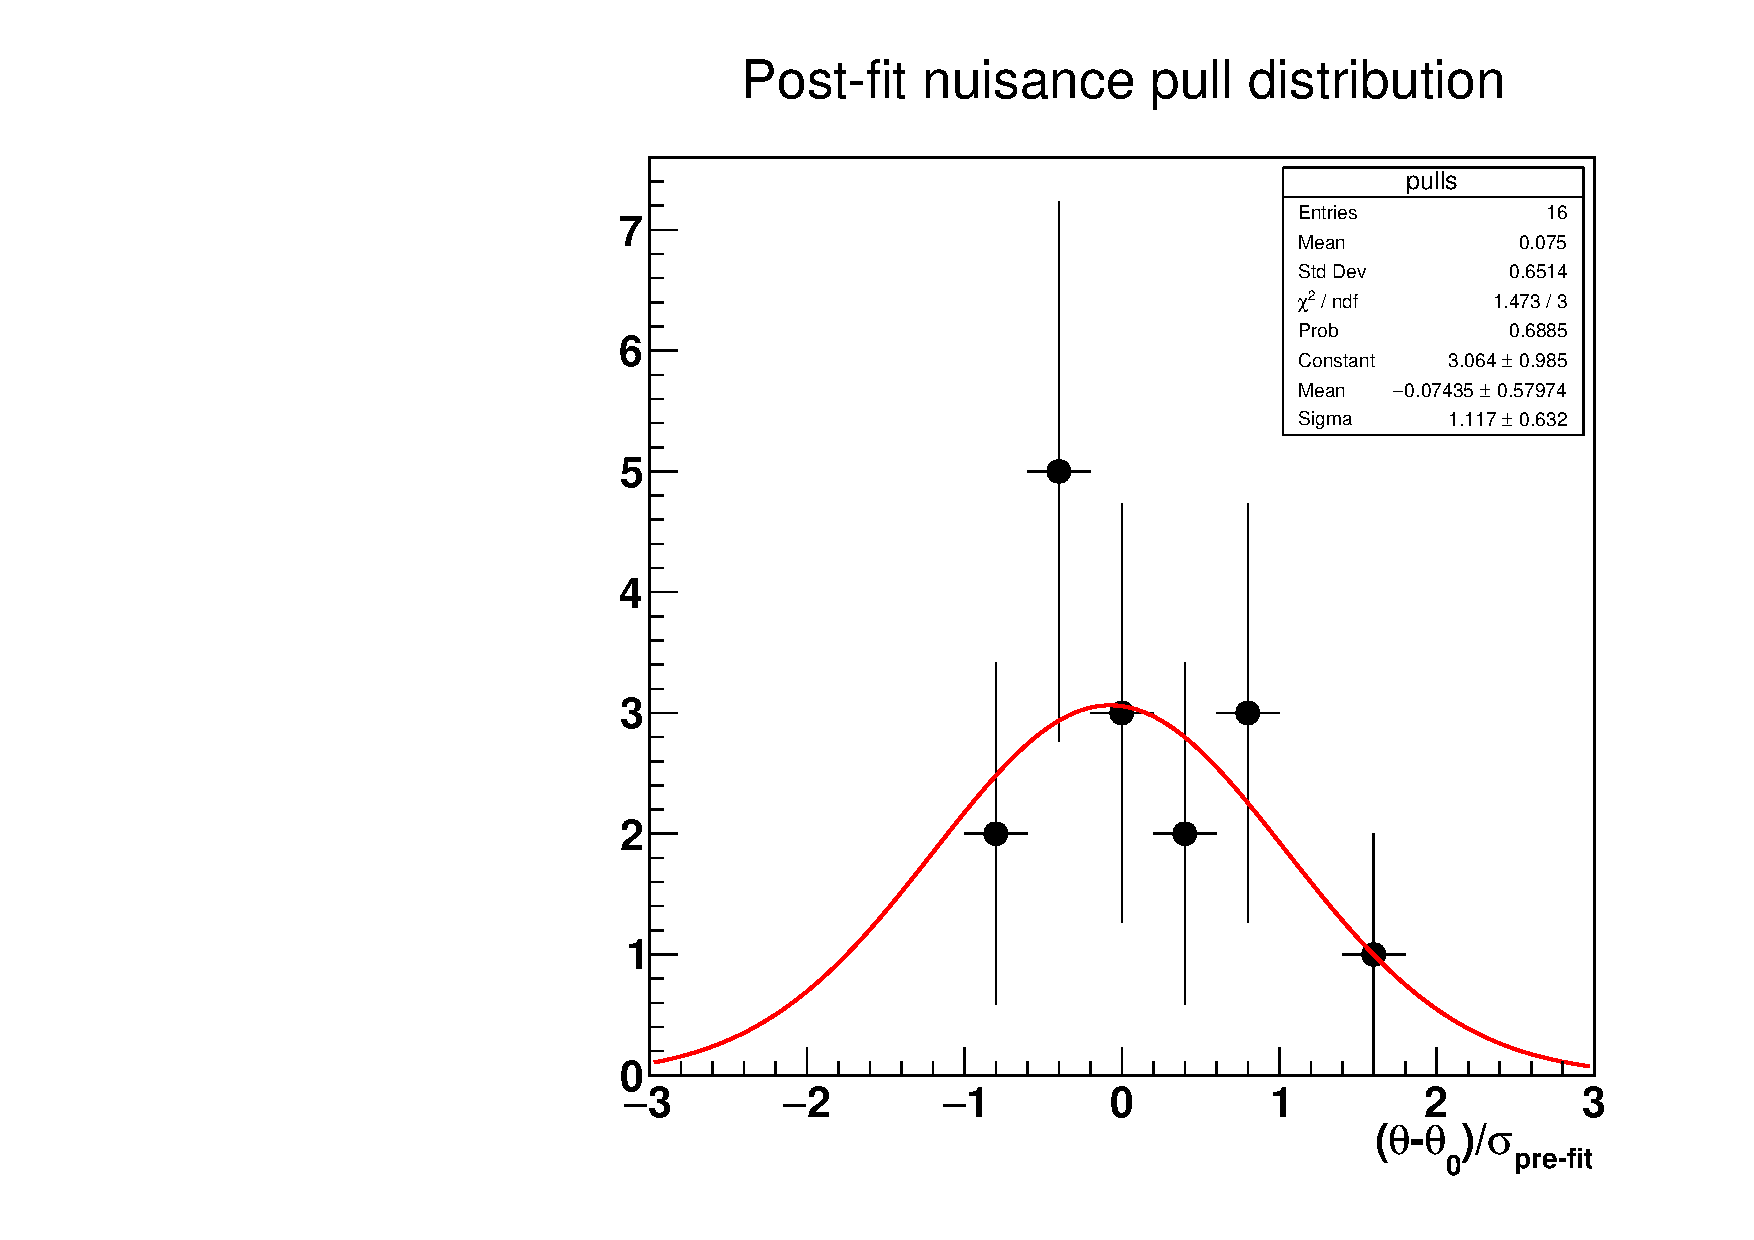
\includegraphics[scale=0.5]{figures/results/nuisancePulls.pdf}
\caption{The distribution of pulls for each background nuisance parameter. Pulls are calculated as the difference between the post-fit value and the pre-fit value divided by the pre-fit uncertainty.}
\label{pre_postfit_param_pulls}
\end{figure}

Finally, we check the observed asymptotic significance of the \stoptolb signal model. As shown in Fig.~\ref{significance_combined_lb}, the observed significance is less than two for all signal points we consider when looking at the combination of all channels as well as each channel individually. We therefore conclude that the observed yields do not constitute a significant excess.

\begin{figure}[hbtp]
\centering
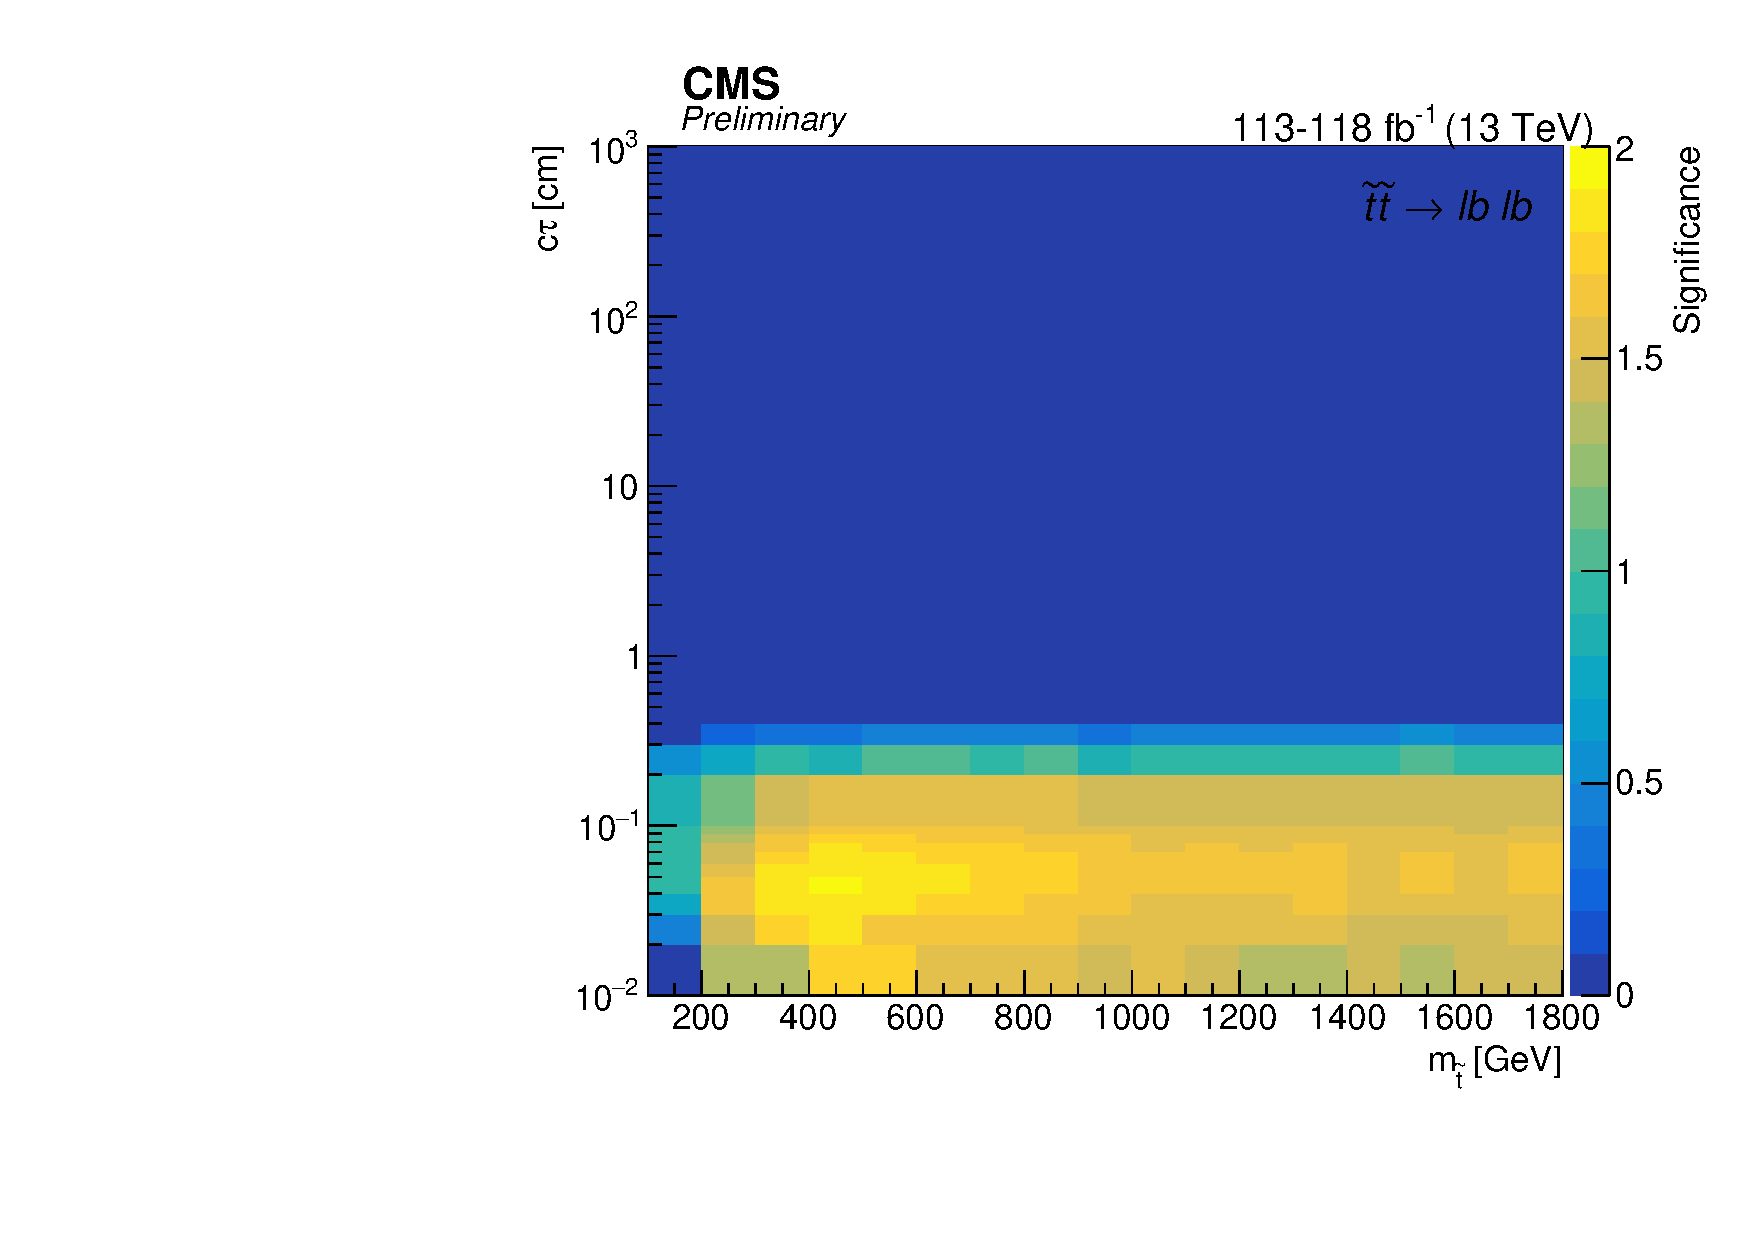
\includegraphics[scale=0.5]{figures/results/significance_combined_lb.pdf}
\caption{The observed asymptotic significances for the \stoptolb process as a function of $\PSQt$ mass and lifetime using the combined results.}
\label{significance_combined_lb}
\end{figure}

\begin{figure}[hbtp]
\centering
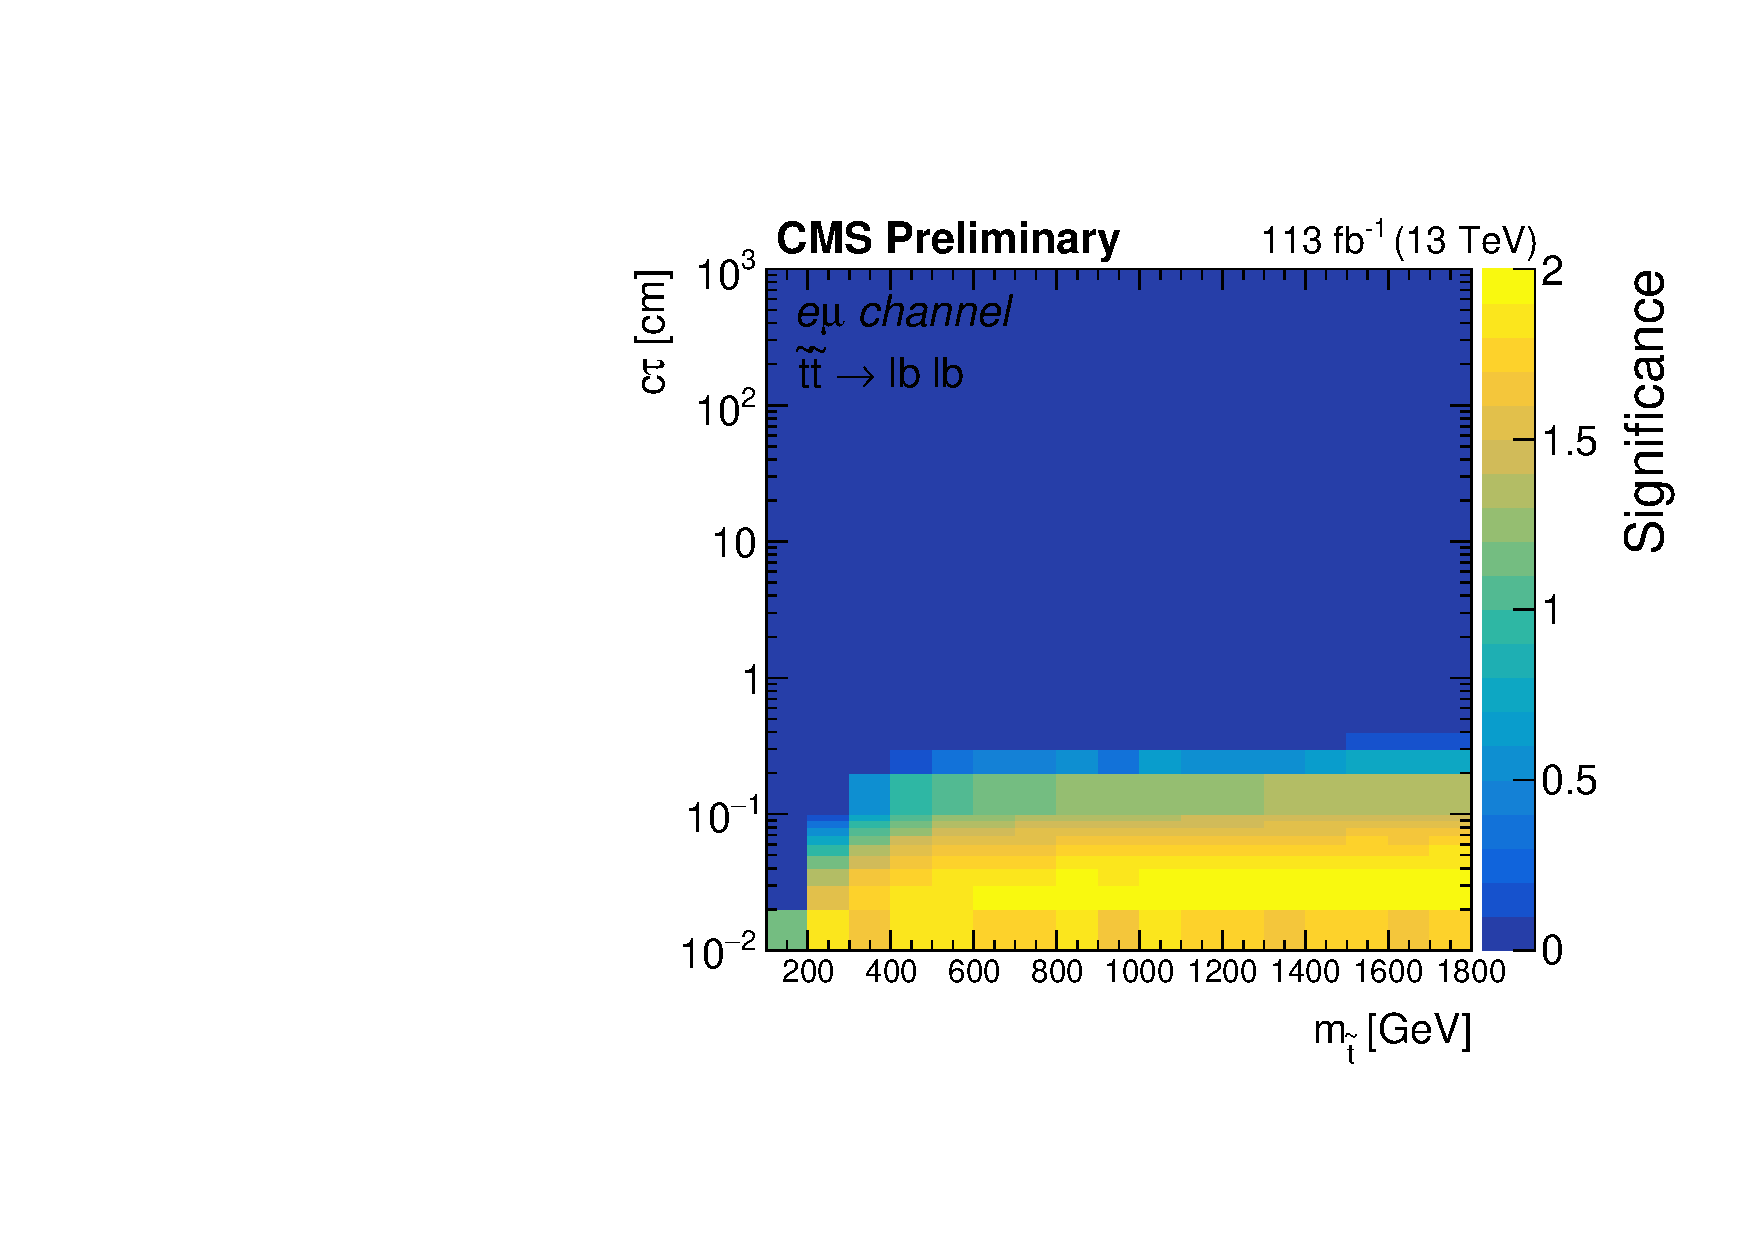
\includegraphics[scale=0.3]{figures/results/emu_lb_significance.pdf}
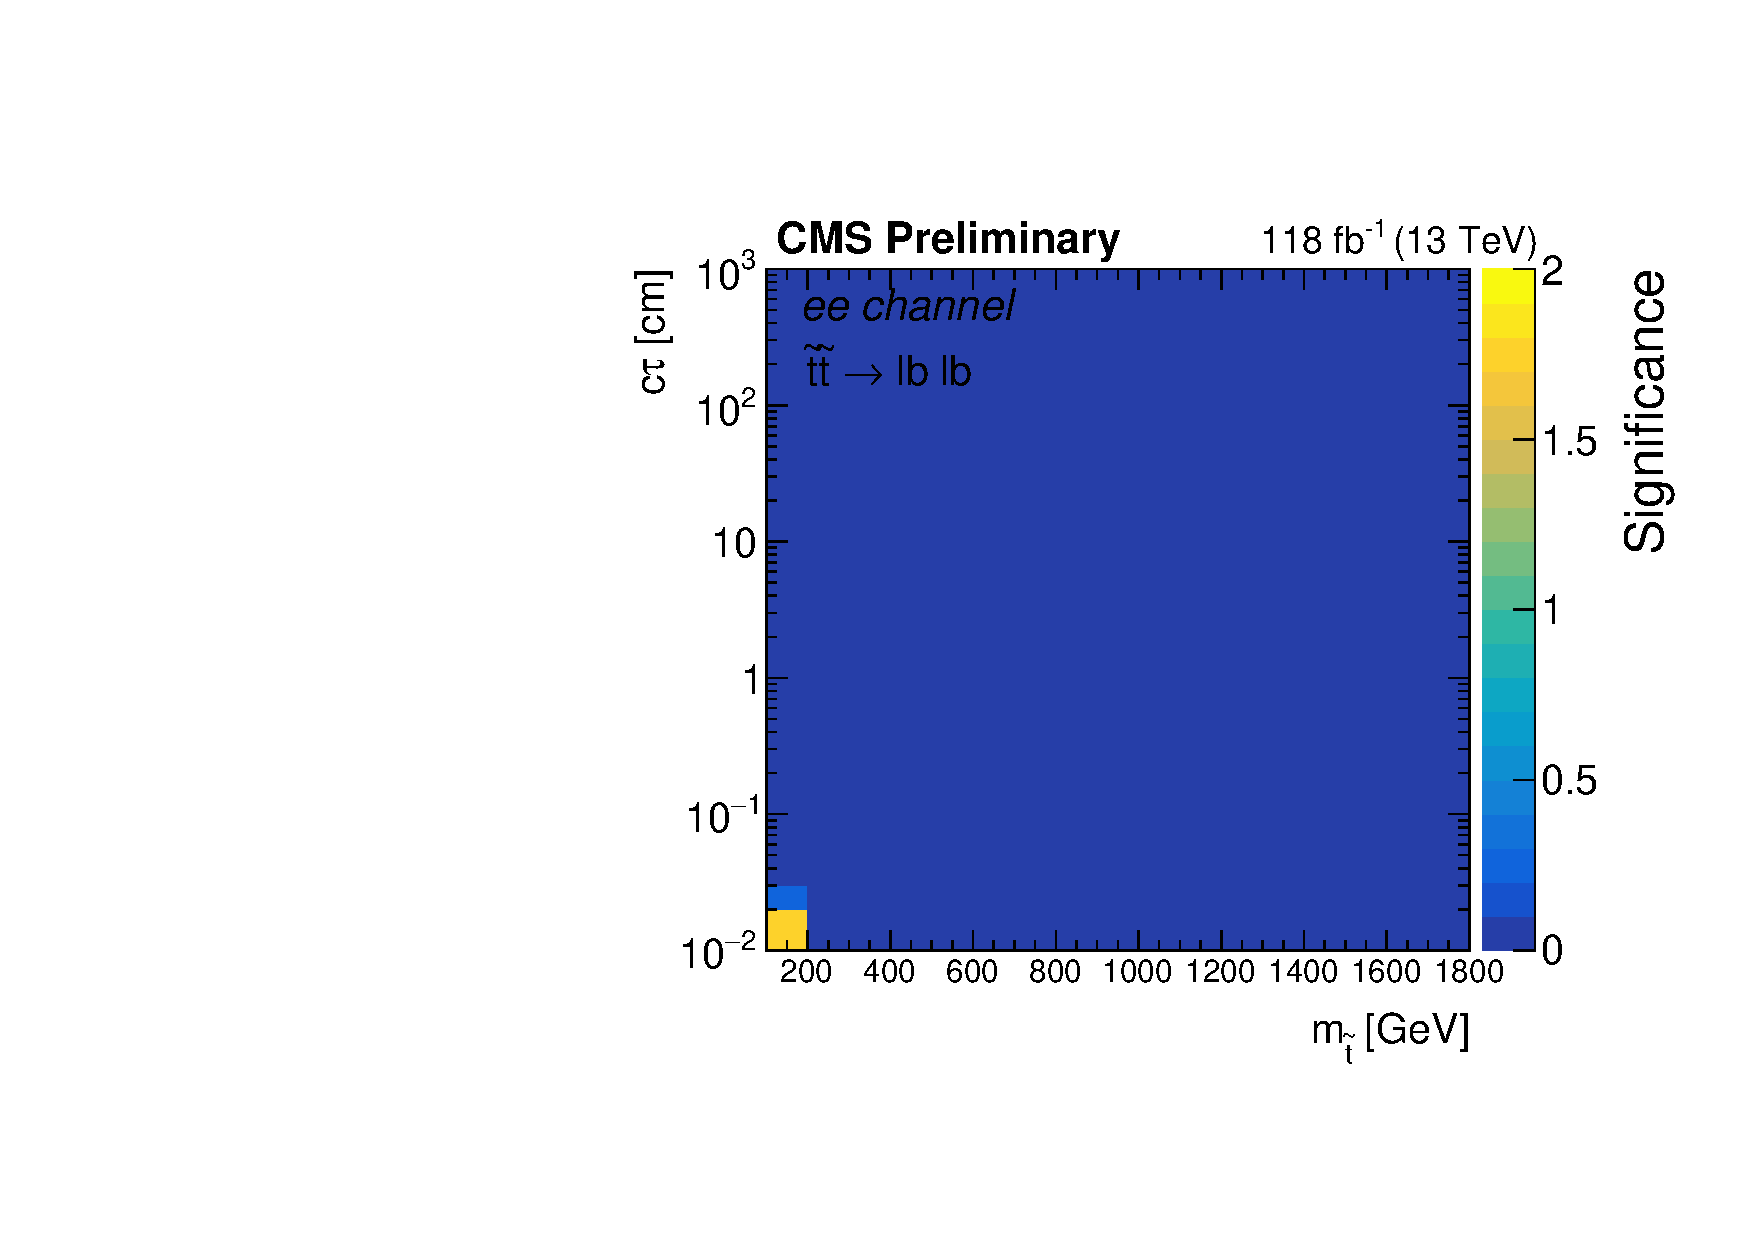
\includegraphics[scale=0.3]{figures/results/ee_lb_significance.pdf}
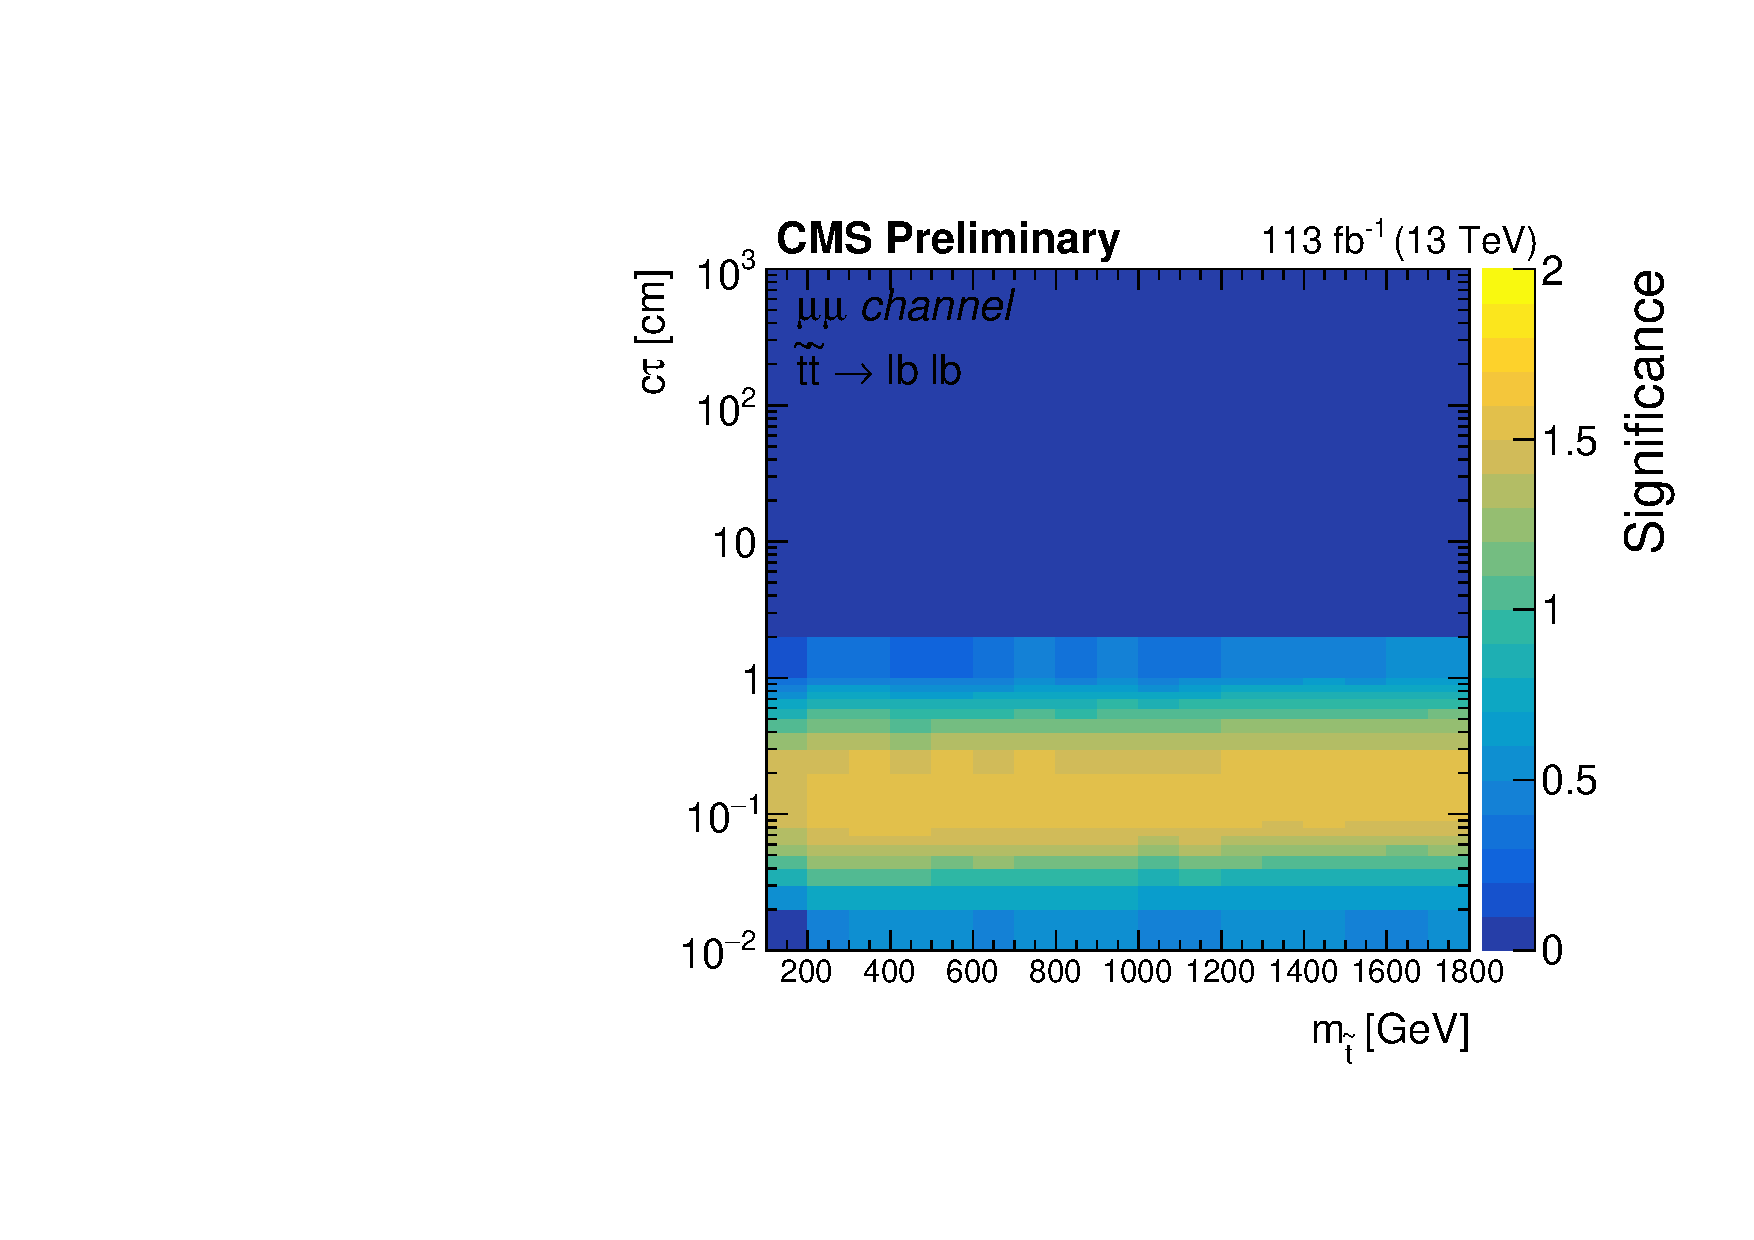
\includegraphics[scale=0.3]{figures/results/mumu_lb_significance.pdf}
\caption{The observed asymptotic significances for the \stoptolb process as a function of $\PSQt$ mass and lifetime in each individual.}
\label{significance_channels_lb}
\end{figure}

\pagebreak